\chapter{Characterizing the interplay between RFA and S1 areas}

\section{Introduction}

When damage occurs to the brain, a disconnection often arises between two previously interconnected brain regions. Specifically, if the primary motor cortex (M1) is damaged, communication with the primary somatosensory cortex (S1) and the spinal cord is disrupted, leading to various impairments. The current standard of care for post-stroke rehabilitation relies on physical therapy. However, emerging electroceutical techniques show promise for restoring lost function by exploiting neural plasticity \cite{Carè2024}.

To evaluate the effectiveness of existing neuromodulation therapies and a novel approach, it is essential to investigate the activity of the RFA and S1 areas. This chapter will show the analyses conducted to understand how the interaction between these spared regions is influenced by an ischemic lesion in the primary motor area (M1, CFA in rats) and subsequent neurostimulation effects. It is crucial to determine whether a new relationship is established between disconnected areas, thereby restoring their communication.

\section{Materials and Methods}

\subsection{Animals}

A total of twenty-six adult male Long-Evans rats (weight: 300-400g, age: 3-4 months; Charles River Laboratories, Calco, LC, Italy) were used in this study. The rats were divided into two main categories: animals with lesions (Lesioned; N=11) and controls (Naïve; N=15)(Figure \ref{fig:Experimental Protocol}). Throughout the entire experimental timeline, the animals were anesthetized. They were randomly assigned to the following groups: (i) Naïve-Sham (animals that did not receive any lesion or stimulation, N=2), (ii) Naïve-Open Loop (animals without lesions that underwent a session of intracortical therapeutic stimulation, N=10), (iii) Lesioned-Open Loop (animals with lesions that underwent a session of Open Loop intracortical therapeutic stimulation, N=11), and (iv) Naïve-Closed Loop (animals without lesions that underwent a session of Closed Loop intracortical therapeutic stimulation, particularly Activity-Dependent Stimulation (ADS), N=3)(Figure \ref{fig:Experimental Protocol}). Animals assigned to the Open Loop treatment randomly received one stimulation type between Exponential, Repeated, and Shuffled. The experimental procedures were conducted at the Animal Facility of the Italian Institute of Technology (IIT), Genova, Italy. The Italian Ministry of Health and Animal Care (Italy: authorization ID 509/2020-PR) approved all experiments conducted in this study.

\subsection{Surgical Procedure}

Anesthesia was induced by placing the rat into a vaporizing chamber and administering gaseous isoflurane (5\% at 1 lpm). Surgical anesthesia was achieved by injecting ketamine (80-100 mg/kg IP) and xylazine (5-10 mg/kg). Anaesthesia was maintained throughout the entire surgical procedure and the registration/stimulation session with repeated bolus injections of ketamine (10-100 mg/kg/hr IP or IM) as needed. Subsequently, the rat was securely positioned in a stereotaxic frame, and continuous monitoring of vital parameters was maintained throughout the entire procedure. The surgical process commenced with the application of lidocaine cream (a topical analgesic), followed by a midline skin incision spanning rostro-caudally between 6 mm rostral to bregma and 5 mm distal to the atlanto-occipital junction the skull. The muscles of the neck overlying the Cisterna Magna or between the upper vertebrae were reflected, and a laminectomy was successfully performed on the spinal dura, facilitating the drainage of cerebrospinal fluid (CSF) to mitigate brain edema during and after the craniotomy.

Using stereotaxic measurements \cite{Kleim2003} +3.5, +2.5 AP, and –1.25, +4.25 ML, burr holes (3 mm diameter) were carefully created over the primary somatosensory area (S1) and rostral forelimb area (RFA). Once the skull was exposed, the dura mater was removed from both burr holes to allow for the insertion of two four-shank, sixteen-contact site electrodes, placed at a depth approximately of 1500 µm (1-1.5 M$\Omega$ impedance, A4x4-3mm-100-125-703-A16, NeuroNexus)

In the lesion group (i.e., Lesion), six 0.7-mm diameter holes were drilled into the skull over the left hemisphere (contralateral to the preferred forelimb) in the area corresponding to the caudal forelimb area (CFA; the M1 forelimb representation analogue in rats) as follows: +2.5, +1.5, +0.5 AP +2.5, +3.5 ML from bregma.
An ischemic injury was then induced in CFA by intraparenchymal injection of Endothelin-1 (ET-1; Merk Life Science S.r.l., Italy, 0.3 µg ET-1 dissolved in 1 µl saline or 1 mg ET-1 dissolved in 3.33 ml saline), a potent vasoconstrictor, 1.5 mm below the pial surface in each of the 6 holes over CFA \cite{Gilmour2005}. The spread of ET-1 with this procedure is confined to an area of 0.5 mm diameter; injections were placed to produce a continuous CFA infarct while leaving RFA and S1 intact \cite{Fang2010}.

\subsection{Experimental Protocol}

As described in the Animals section, four main experimental groups were used: (i) Naïve-Sham, (ii) Naïve-Open Loop, (iii) Lesion-Open Loop and (iv) Naïve-Closed Loop. 

The experimental timeline (Figure \ref{fig:Experimental Protocol}) mainly comprised three recording phases: before the lesion (PreL), between the lesion and stimulation (PoL), and after the stimulation (PoS). The first phase included a sequence of 20-minute spontaneous activity, 10-minute connectivity mapping, and another 10-minute spontaneous activity recordings. The second phase consisted of 20-minute spontaneous activity recording followed by 10-minute connectivity mapping recording. The final phase comprised 10-minute connectivity mapping recording followed by 20-minute spontaneous activity recording.

\begin{figure}[htp]
    \begin{center}
    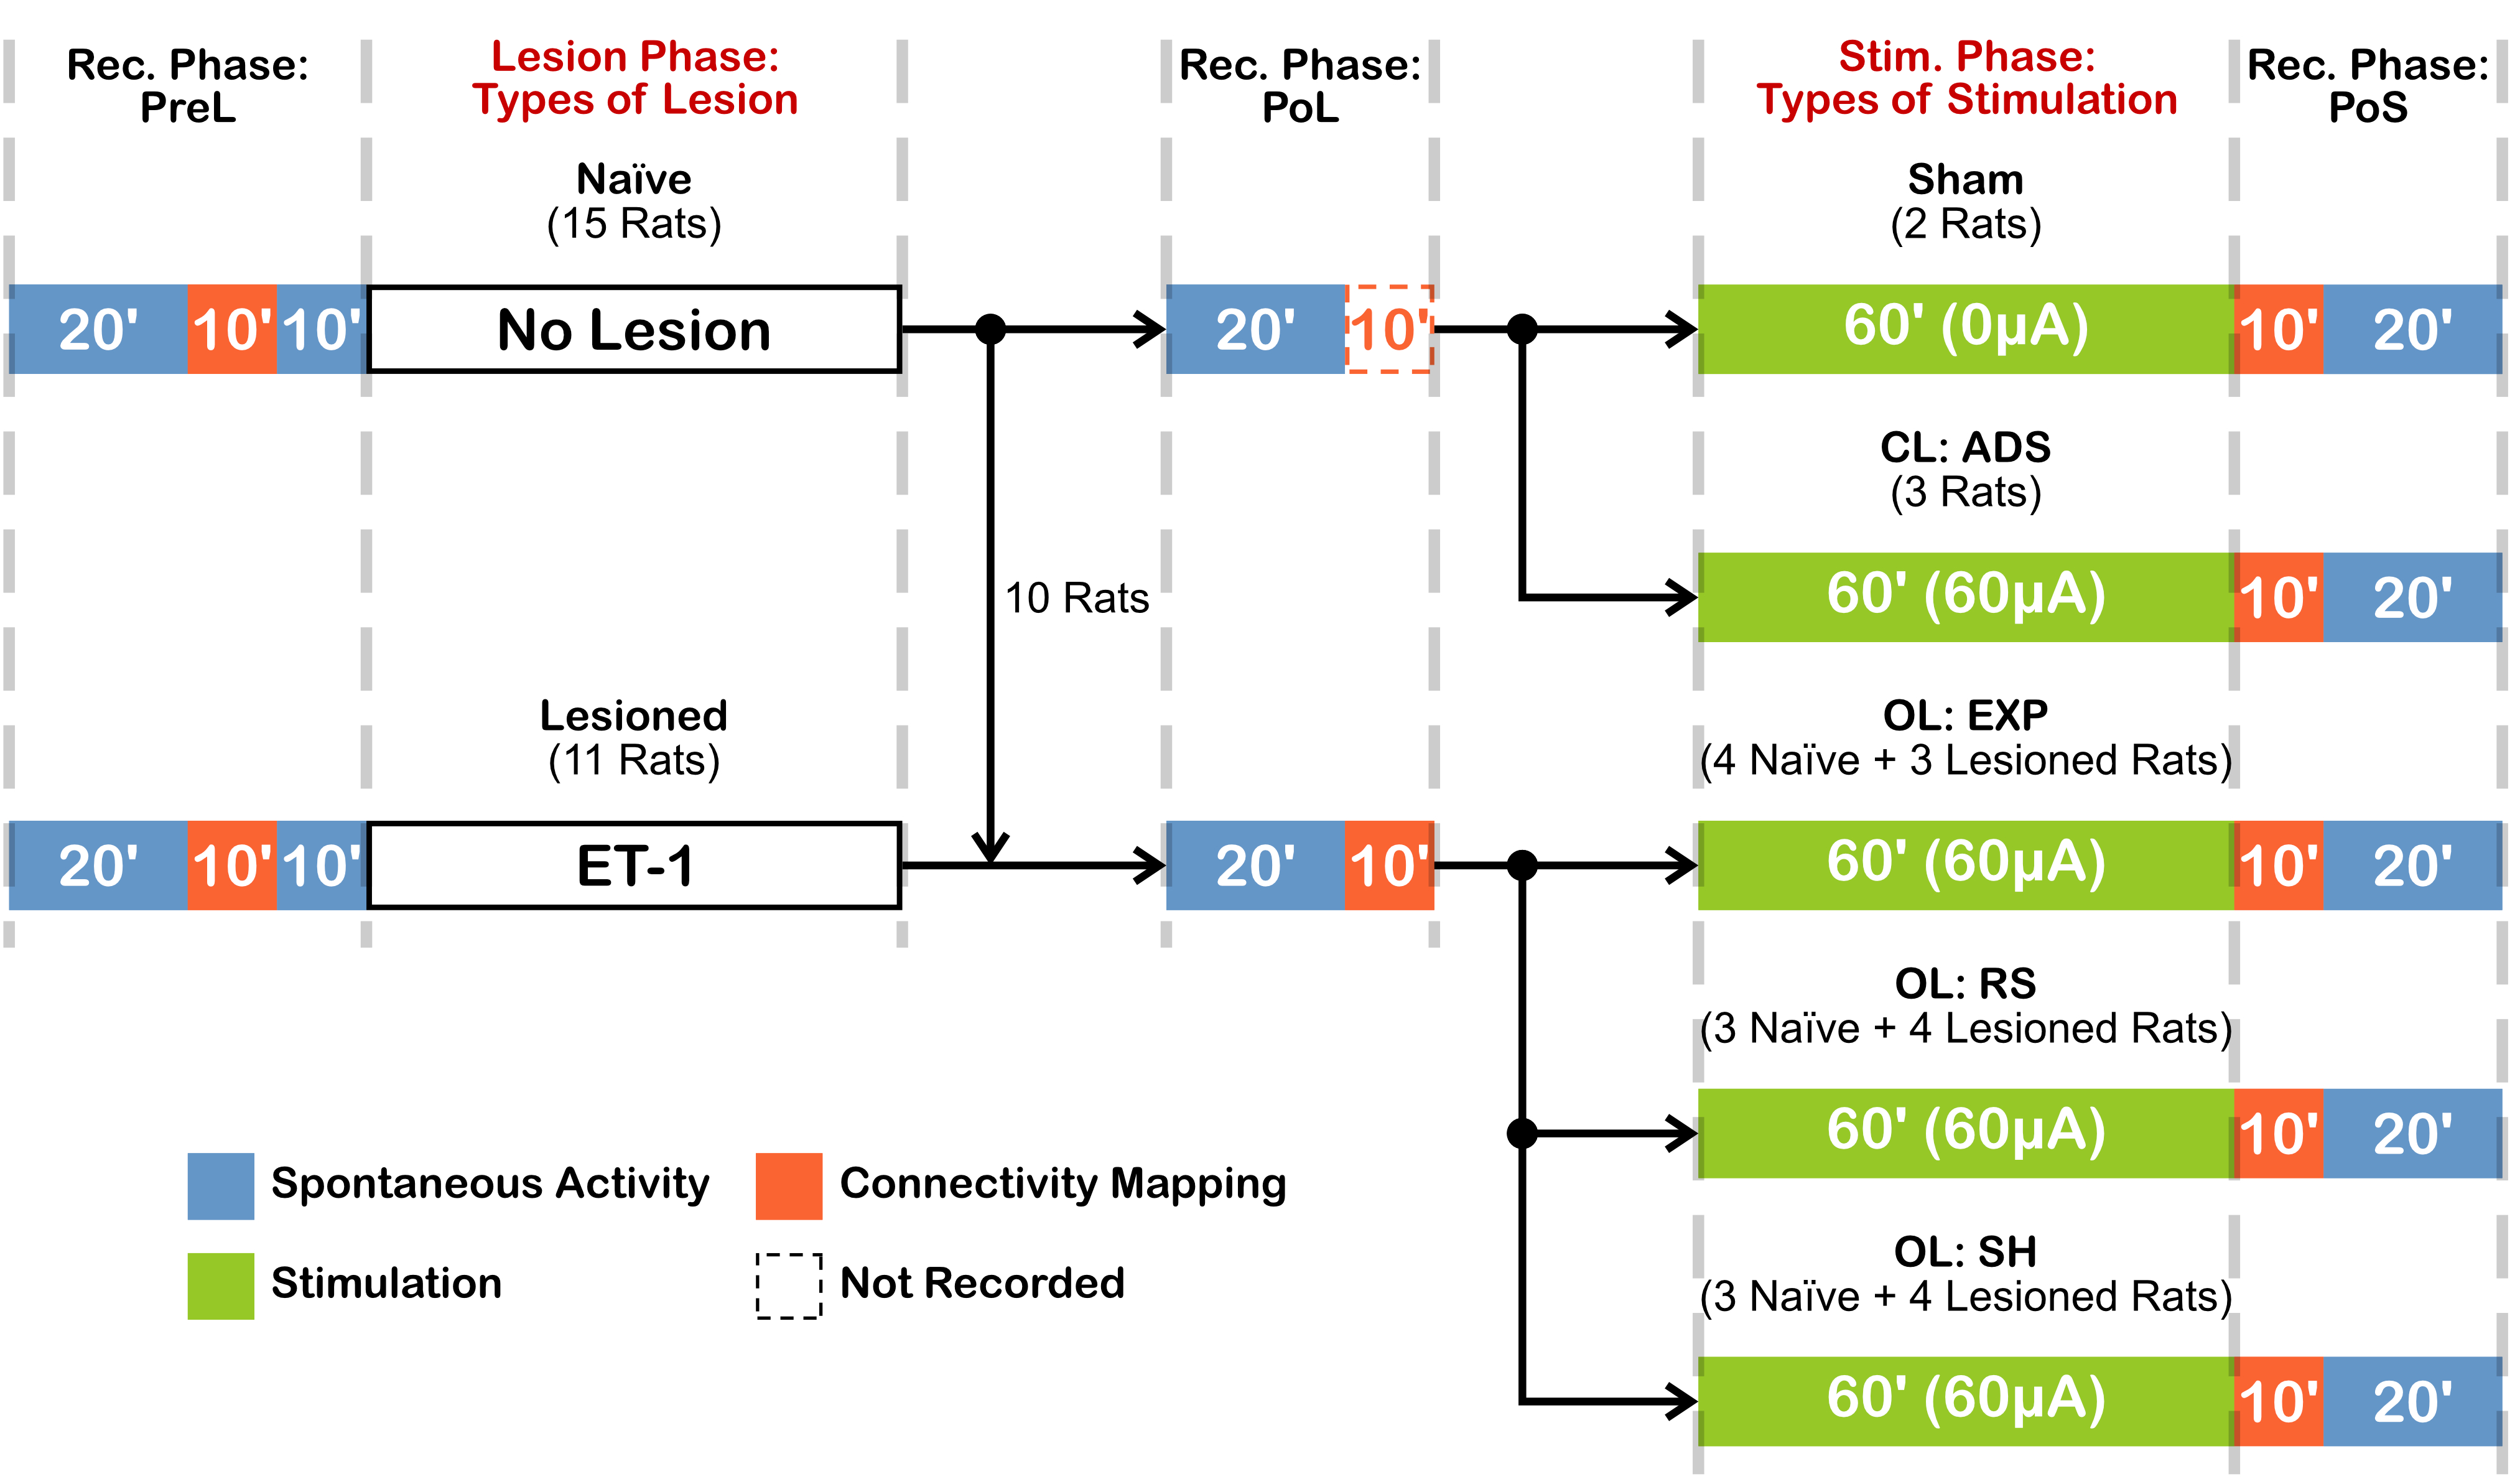
\includegraphics[width=\linewidth]{Figure/Experimental Protocol/Experimental Protocol.jpg}
    \end{center}
    \caption{Experimental timeline. All the phases of the experiment are depicted in the image, including the distribution of rats among the various experimental groups. Twenty-six rats were initially divided into two groups (Naïve and Lesioned), and then further subdivided into five groups based on the type of stimulation they received (Sham, Closed Loop: Activity Dependent Stimulation (CL: ADS), Open Loop: Exponential (OL: EXP), Open Loop: Repeated (OL: RS), Open Loop: Shuffling (OL: SH)) for a total of eight groups (Naïve-Sham, Naïve-CL:ADS, Naïve-OL: EXP, Naïve-OL: RS, Naïve-OL: SH, Lesioned-OL: EXP, Lesioned-OL: RS, Lesioned-OL: SH). All groups underwent the same Pre-Lesion (PreL) and Post-Stimulation (PoS) phases, but only those subjected to an open loop stimulation protocol underwent connectivity mapping recording during the Post-Lesion (PoL) phase.}
    \label{fig:Experimental Protocol}
\end{figure}

Extracellular signals have been continuously sampled at a rate of 25 kHz using standard, commercially available neurophysiological hardware (Intan RHS, Intan technologies LLC) and for better efficiency in the data processing step, data were saved in blocks of 10-min recordings each.

In the Naïve groups, a ‘No Lesion’ period was considered, which lasted approximately 1 hour. In the groups that received the stimulation (i.e. Naïve-Open Loop, Lesion-Open Loop and Naïve-Closed Loop) 1 hour of stimulation (e.g. Exponential, Repeated, Shuffling and Activity-Dependent Stimulation) was recorded, while in the Sham group was recorded one more spontaneous session (i.e. Sham). In all the experiments, the stimulation pulse was designed to be a single squared 60 µA biphasic, cathodal-leading pulse (200 µs positive, 200 µs negative), however in the Sham animals the pulse current was set to 0 µA.

Moreover, only in the groups that received an Open Loop stimulation, a Post-Lesion (PoL) Connectivity mapping recording was actually performed (Figure \ref{fig:Experimental Protocol}).

\subsubsection{Connectivity mapping phase}

An impedance analysis was performed and according to the lowest value (200-300 k$\Omega$), two single channels from S1 were selected to deliver the stimulations. Two different channels have been chosen to investigate whether the effects of stimulation could be location-dependent. In addition, two different frequencies were tested to explore potential variations in response speed. Specifically, the protocol for the connectivity mapping consisted of two recording steps to investigate evoked responses. (i) a stimulus was delivered every second for 1 minute (corresponding to a sample rate of 1 Hz), through two different channels, and a 30-sec of ‘no stimulation’ was recorded between the two channels. (ii) a stimulus was delivered every 5 seconds for a total of 30 times (resulting in a sample rate of 0.2 Hz), through two different channels, and a 30-sec of ‘no stimulation’ was recorded between the two channels.

\subsubsection{Stimulation phase}

An impedance analysis was performed on the S1 electrode and the single channel with the lowest impedance value (approximately 0.2 M$\Omega$) was chosen for delivering the stimulation.

For all the open loop stimulation methods, the following steps were followed: (i) During the first spontaneous activity recording, one of the sixteen channels in RFA was selected based on visual observation of spike amplitudes and signal to noise ratios; (ii) the timestamp was extracted; (iii) subsampling was done at a frequency of 1 kHz in order to load the stimulation vector onto Simulink; (iv) the stimulation pattern was created according to the chosen method, described above; (v) the stimulation was controlled using a model loaded onto Simulink, which was delivered through a breakout box connected to the INTAN RHS Stim/Recording System (intantech).

For the closed loop stimulation method, the first step followed was the same as the open loop methods, while the second step involved setting a channel-specific threshold in the Intan software, to act as the trigger for activity-dependent stimulation (ADS).

\subsection{Stimulation paradigms}

All the animals of the Lesion group and 10 Naïve rats were randomly assigned to one of the four stimulation groups (see Figure \ref{fig:Experimental Protocol}):
\begin{itemize}
    \item \textbf{OL: Exponential Stimulation:} the mean firing rate of the extracted time stamps from the first 20-min of the healthy spontaneous activity recorded before the lesion was used to design a new spike sequence according to a pre-defined/mathematical distribution, e.g., exponential distribution (Mathworks); 
    \item \textbf{OL: Repeated Stimulation:} the first 10-min of the healthy spontaneous activity recorded before the lesion (i.e., PreL) on a selected channel in RFA were looped six times to deliver a stimulation pattern lasting an hour \cite{Zullo2012};
    \item \textbf{OL: Shuffling Stimulation:} a new spike sequence of the duration of interest was generated according to a data-driven ISI, based on data acquired from a reference network;
    \item \textbf{CL: Activity-Dependent Stimulation:} a single stimulation pulse was delivered to a selected channel on the S1 probe each time the pre-configured threshold was crossed. To prohibit feedback from stimulus-evoked RFA spikes and stimulus artifacts from triggering stimulation, a blanking period (28 ms) followed each stimulus limiting the maximum stimulation rate to roughly 35 Hz.
\end{itemize}

\subsection{Data and Statistical Analyses}

\subsubsection{Preprocessing}

All the preprocessing of the in-vivo recordings was performed in MATLAB (The MathWorks, Natick, MA, USA). The ePhys data underwent preprocessing through a custom MATLAB pipeline. Briefly, data was formatted into a MATLAB-readable structure and organized on a per-channel basis. Subsequently, a 4th order elliptic bandpass filter (300-3000 Hz) was applied to eliminate low-frequency components in the signal. A power-based spike detection algorithm known as Stationary Wavelet-based Teager Energy Operator (SWTTEO) \cite{Lieb2017} was employed to identify spikes from the filtered data. The SWTTEO involved two levels of Stationary Wavelet Transform (SWT) followed by the use of the Teager Energy Operator (TEO). The TEO outputs were smoothed, summed, and their combination was thresholded. Multiunits were later sorted using a mixture of skew-t distributions on PCA-extracted features, following the approach outlined in \cite{Toosi2021}. Peaks that clearly corresponded to noise were excluded at this stage by assignment to a “noise” or “non-neural” source cluster.

\subsubsection{Post-Stimulus Time Histogram (PSTH)}

The evoked activity was assessed by computing the post-stimulus time histogram (PSTH) using an adapted version of a custom software package (SPYCODE) (Bologna et al. [2010]). A time window of 800 ms, a bin size of 4 ms and a blanking period of 0.4 ms were chosen. Two separate PSTHs and the corresponding areas under the PSTH curve were calculated for each electrode (multi-unit activity). This separation aimed to distinguish the PSTH generated by the first stimulation channel from the one generated by the second channel (e.g., the first PSTH and area under the PSTH curve considered the first 30 stimuli).

\subsubsection{Statistical Analysis}

The statistical analysis was performed in MATLAB as well. For each rat two mean values were considered: one for the PSTH areas obtained with a stimulation frequency of 1Hz and one for the PSTH areas obtained with 0.2Hz. To identify differences in the PSTH areas between all the phases of the experimental protocol (PreL, PoL and PoS) a one-way ANOVA test was performed. P-values were considered significant for $p<0.05$.

\section{Results}

To analyze how the lesion and the subsequent stimulation phase affect the networks, stimulations at two different frequencies (1 Hz and 0.2 Hz) were delivered to map the recorded areas. The PSTH analysis of the connectivity mapping stimulations was used to assess the intra- and inter-area evoked responses.
In Figure \ref{fig:RasterPSTH}, the activity elicited by the 0.2Hz stimulus is illustrated. This activity was recorded in one of the channels from both the RFA and the S1 areas of a representative animal that received shuffled stimulation after the lesion. Additionally, Figure \ref{fig:PSTH} depicts a representative Post-Stimulus Time Histogram (PSTH) of the evoked response after the 0.2Hz stimulus in the same animal.

\begin{figure}[htp]
    \begin{center}
    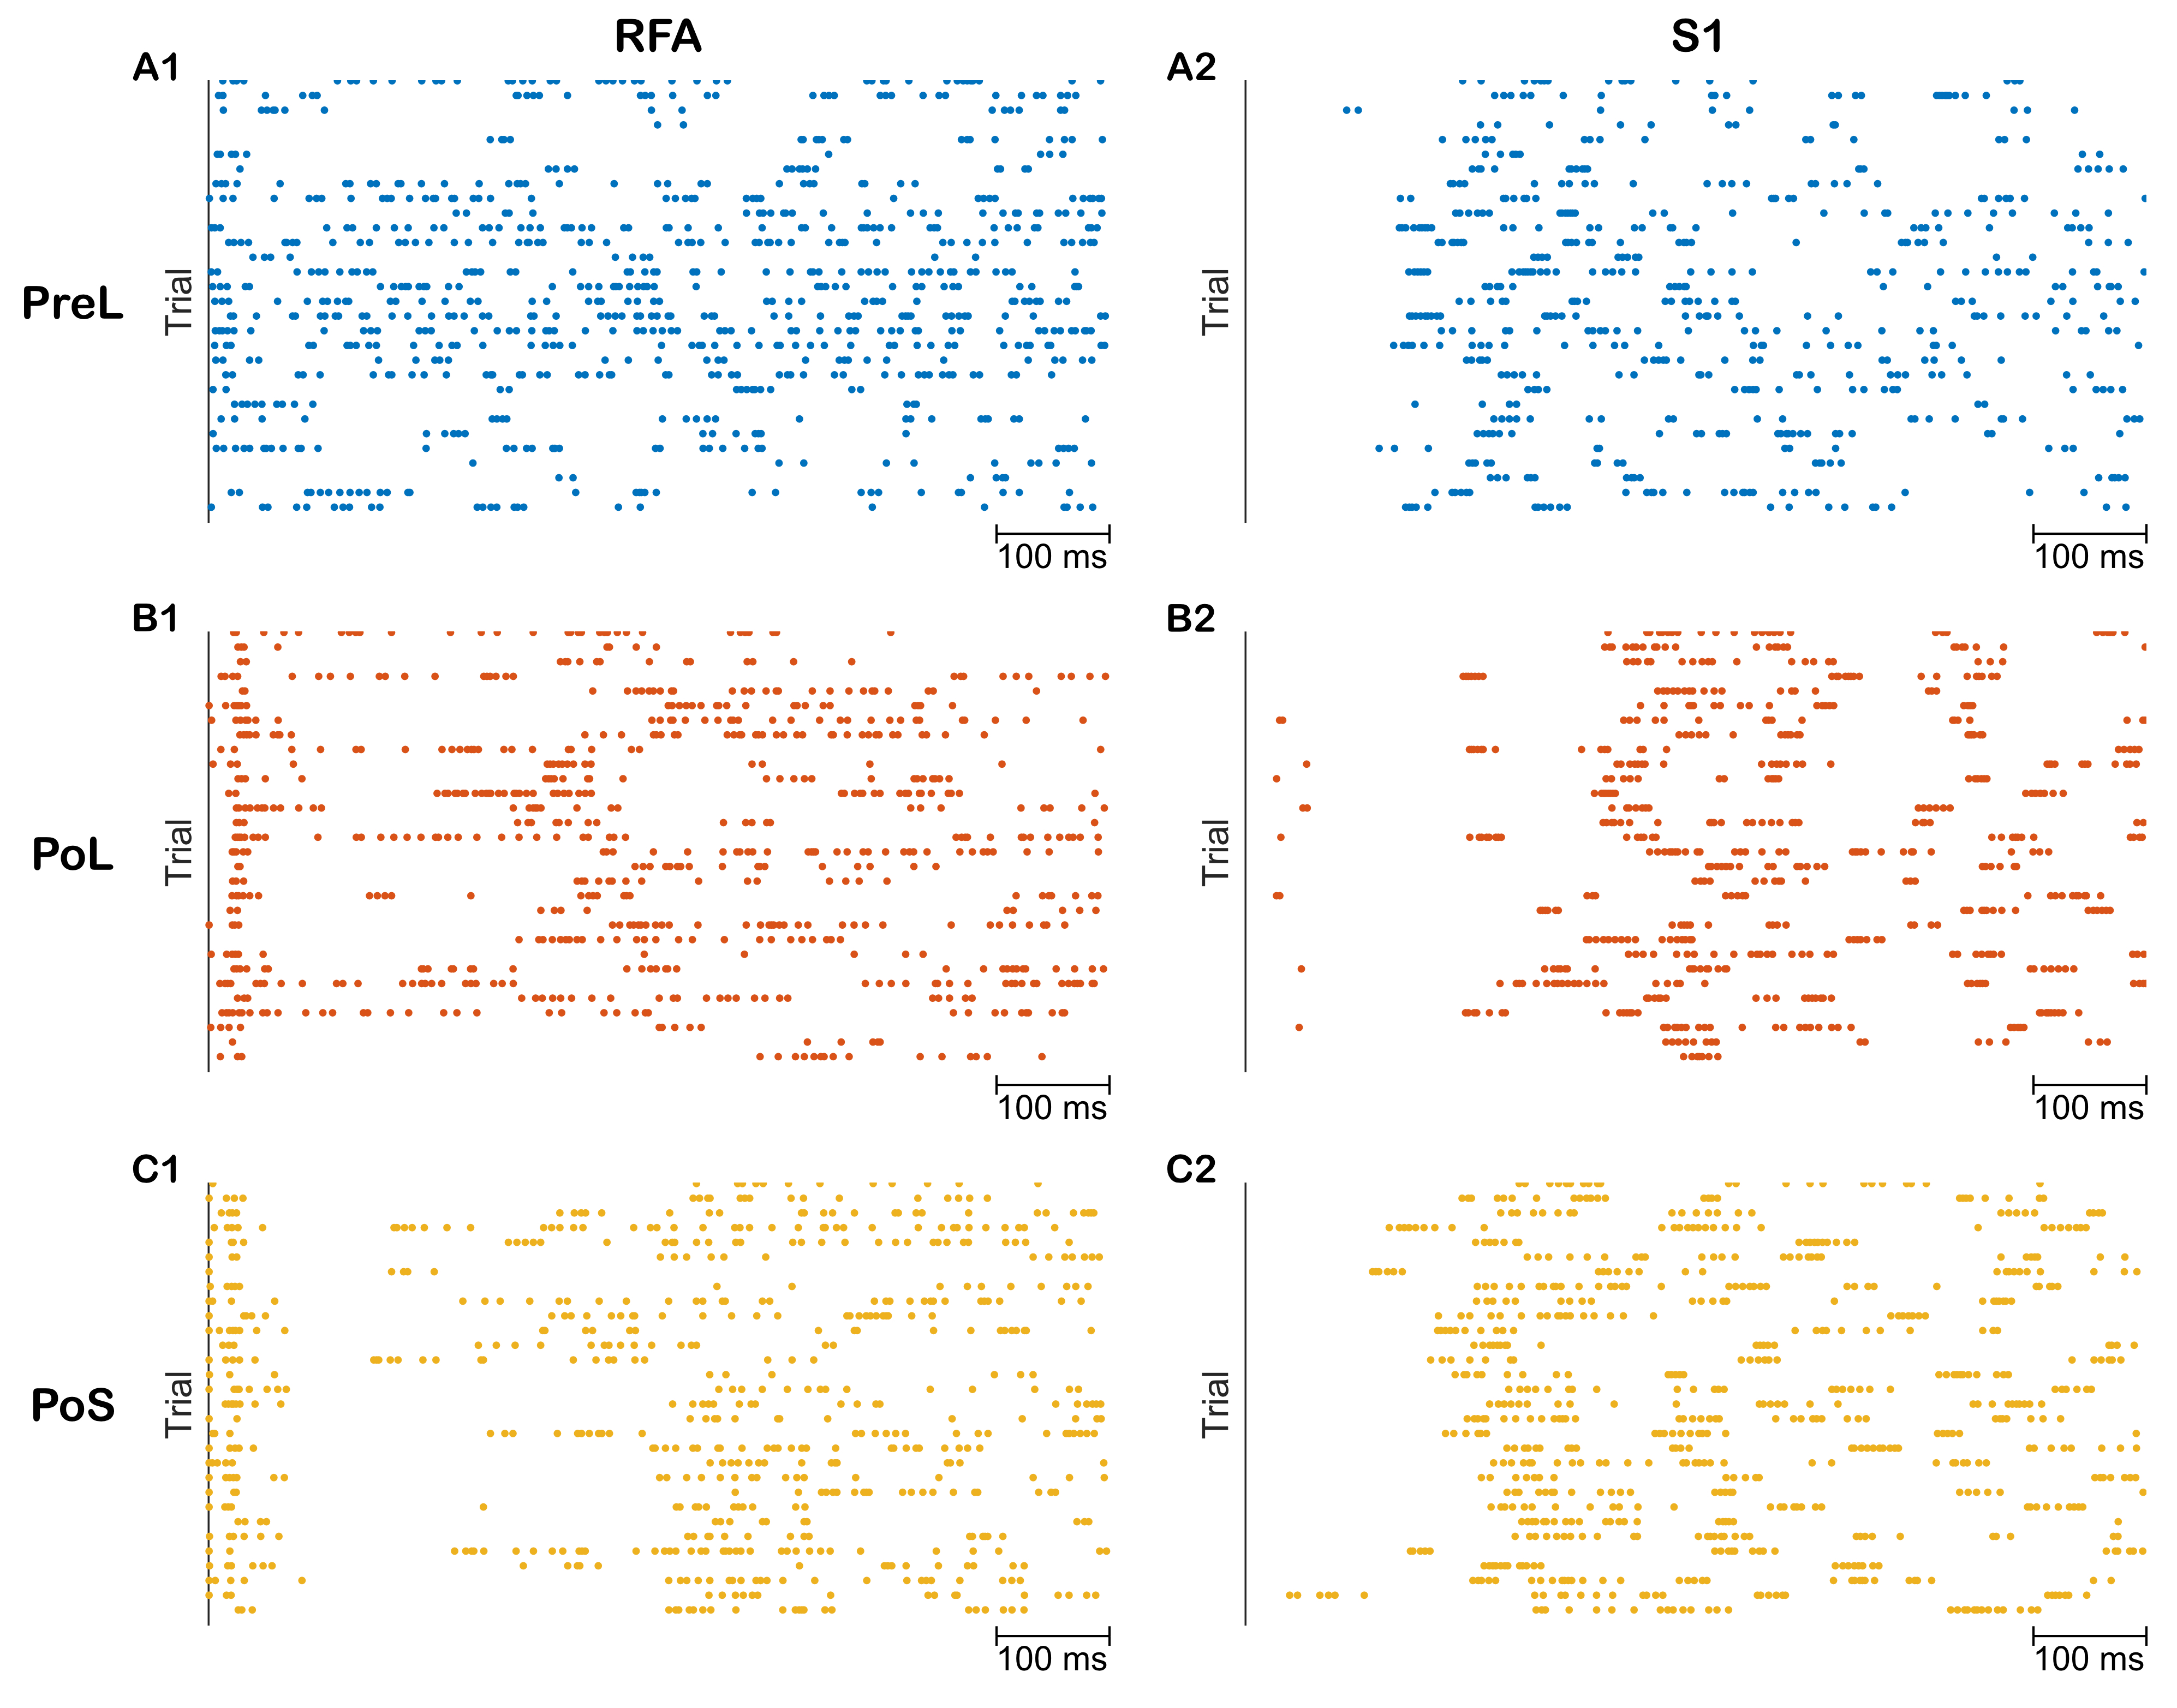
\includegraphics[width=\linewidth]{Figure/rasterplot PSTH/RasterPSTH.jpg}
    \end{center}
    \caption{Firing Activity Evoked by the Connectivity Mapping Stimulations. (A) 800-ms raster plots depict the recorded activity in the RFA (left) and S1 (right) areas after the connectivity mapping stimulation before the lesion (PreL, blue). (B) 800-ms raster plots illustrate the recorded activity in the RFA and S1 areas after the connectivity mapping stimulation following the lesion (PoL, orange). (C) 800-ms raster plots show the recorded activity in the RFA and S1 areas after the connectivity mapping stimulation following the delivery of personalized stimulation (PoS, yellow).}
    \label{fig:RasterPSTH}
\end{figure}

\begin{figure}[htp]
    \begin{center}
    \includegraphics[width=\linewidth]{Figure/PSTH/PSTH.jpg}
    \end{center}
\end{figure}
\begin{figure}[p!]
    \caption{(figure in the previous page) PSTH graphs. Each graph represent the PSTH of a single channel before (blue) and after (orange) the lesion, and after the stimulation (yellow). On the top, the PSTHs in the stimulation area (i.e., S1), and the red square highlights the stimulation channel. On the bottom, the evoked responses in the recording area (i.e., RFA). The channels are spatially ordered as in the arrays. On the x-axis there is the time in seconds, on the y-axis there is the firing rate in spikes per seconds.}
    \label{fig:PSTH}
\end{figure}
\clearpage

\subsection{The effect of the ischemic lesion on the evoked responses}

This analysis was also employed to investigate whether the lesion could be localized and impact some regions more than others. In particular, the area under the PSTH of the Lesioned and Naïve animals that recieved both PreL and PoL connectivity mapping recordings were considered to obtain an overall understanding about the efficacy of the lesion. In Figures \ref{fig:Lesion Effect 0.2Hz} and \ref{fig:Lesion Effect 1Hz}, a more significant decrease in the PSTH area can be appreciated in both areas of the rats that received a lesion compared to those in the Naïve group. In particular, considering the slope of the regression lines, it’s possible to emphasize and evaluate the negative impact of the lesion on the evoked responses. The Naïve group, indeed, exhibits a higher slope than the group that actually underwent the lesion.

\begin{figure}[ht!]
    \begin{center}
    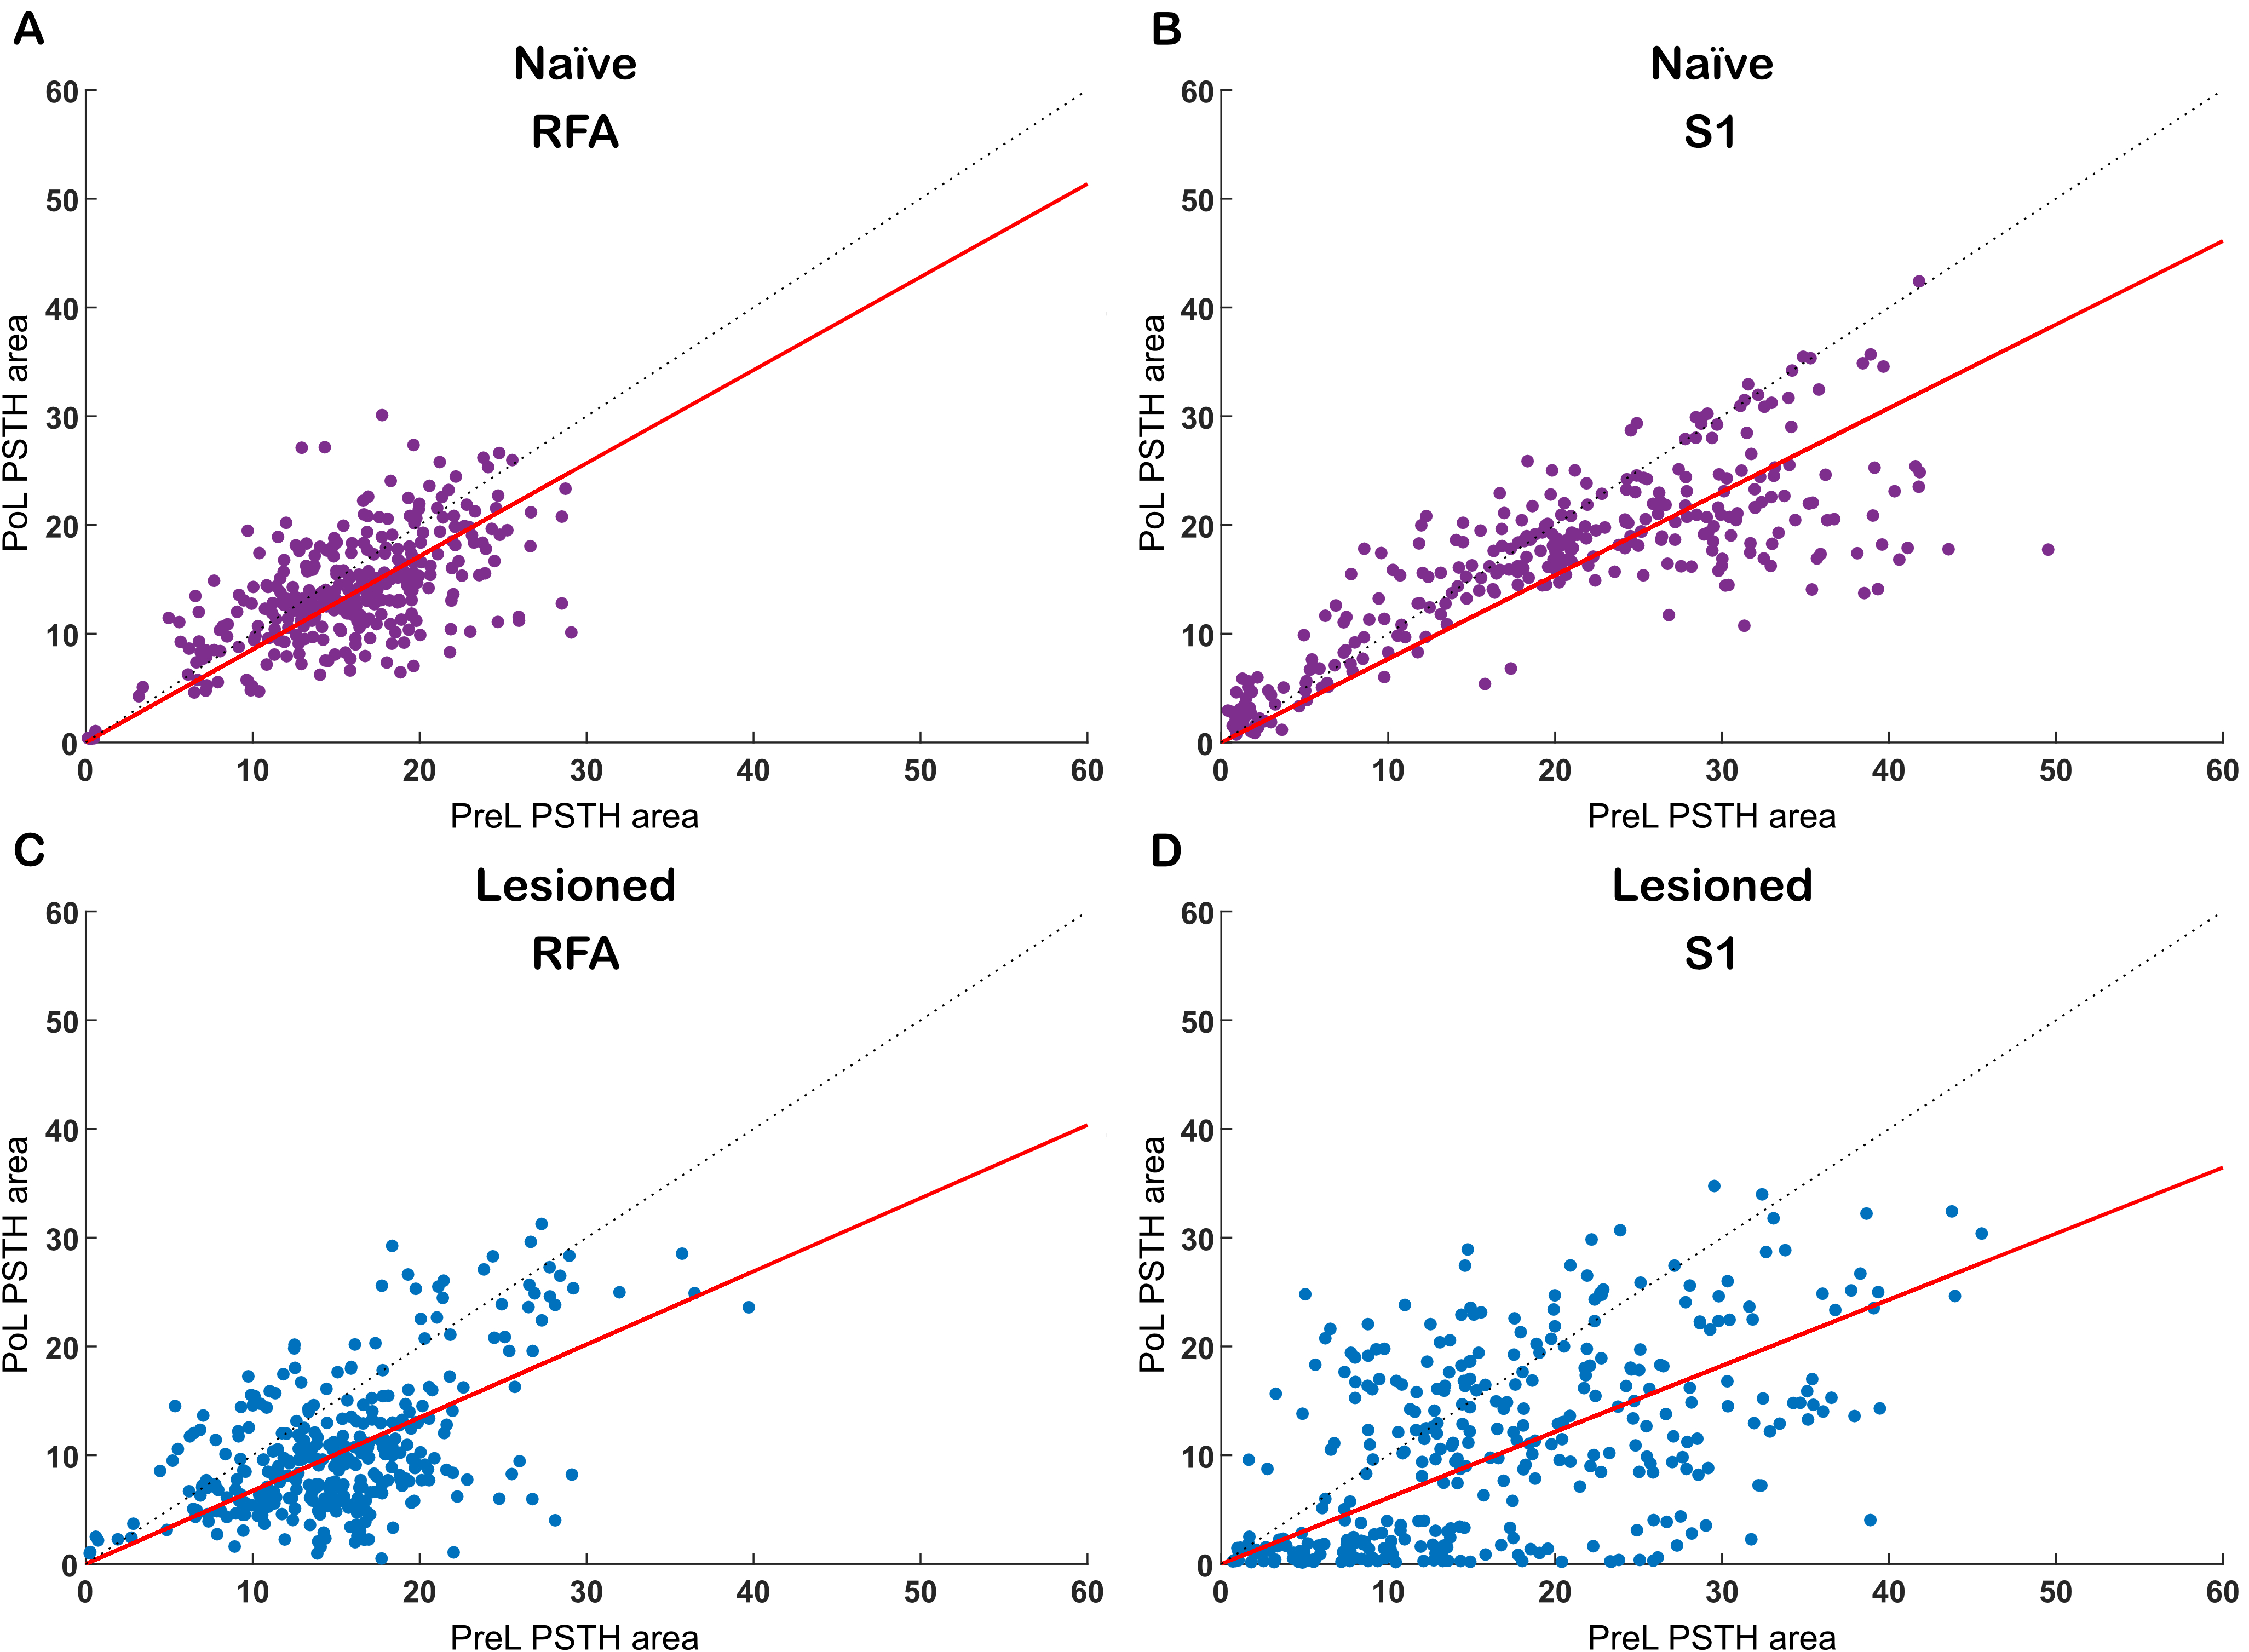
\includegraphics[width=\linewidth]{Figure/Lesion Effect/Lesion Effect 0.2Hz.jpg}
    \end{center}
    \caption{Pre-Lesion and Post-Lesion PSTH area for the 0.2Hz stimulation rate. Left: results in RFA. Right: results in S1. (A, B) On the top: scatterplot of the PSTH area in the Naïve group. (C, D) On the bottom: scatterplot of the PSTH area in the Lesioned group. On the x-axis is showed the Pre-Lesion (PreL) PSTH area and on the y-axis the Post-Lesion (PoL) PSTH area. Each dot represent a channel. The dotted line represents the bisector with a slope of 1. The red line represent the regression line of the dots that pass through the center of axes (slopes: A: 0.86, B: 0.77, C: 0.67, D: 0.61).}
    \label{fig:Lesion Effect 0.2Hz}
\end{figure}

\begin{figure}[ht!]
    \begin{center}
    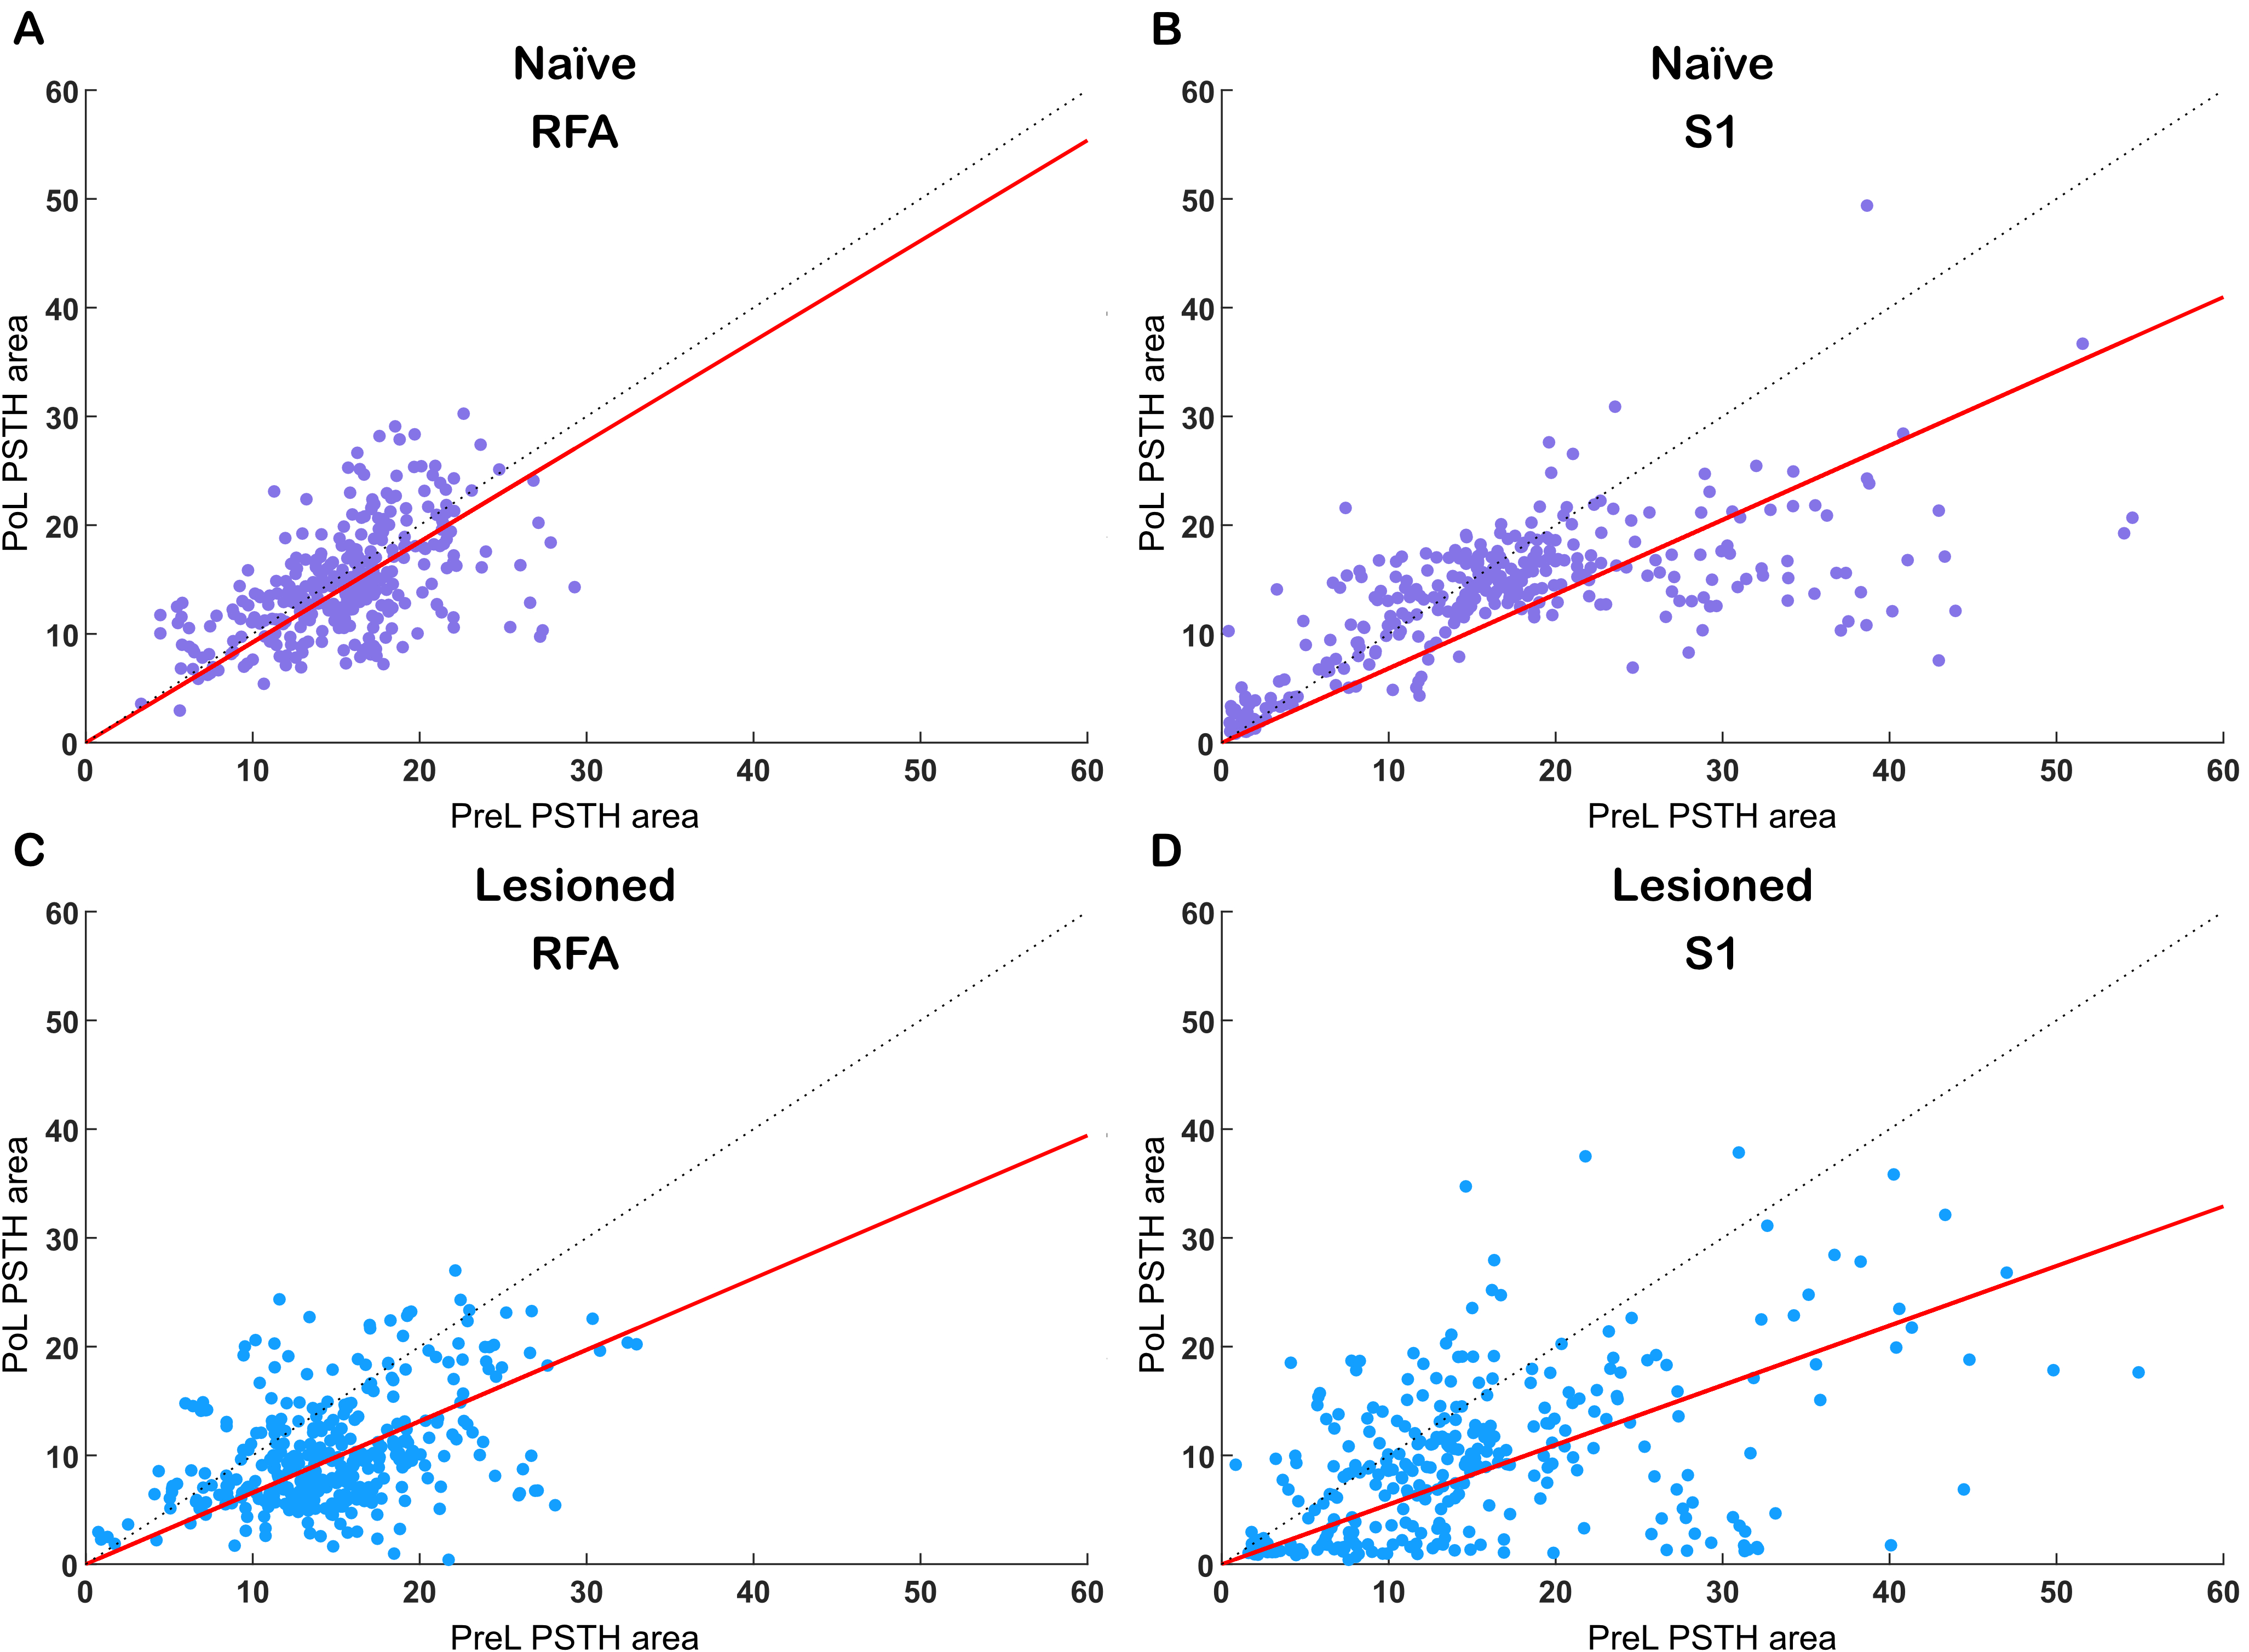
\includegraphics[width=\linewidth]{Figure/Lesion Effect/Lesion Effect 1Hz.jpg}
    \end{center}
    \caption{Pre-Lesion and Post-Lesion PSTH area for the 1Hz stimulation rate. Left: results in RFA. Right: results in S1. (A, B) On the top: scatterplot of the PSTH area in the Naïve group. (C, D) On the bottom: scatterplot of the PSTH area in the Lesioned group. On the x-axis is showed the Pre-Lesion (PreL) PSTH area and on the y-axis the Post-Lesion (PoL) PSTH area. Each dot represent a channel. The dotted line represents the bisector with a slope of 1. The red line represent the regression line of the dots that pass through the center of axes (slopes: A: 0.92, B: 0.68, C: 0.66, D: 0.55).}
    \label{fig:Lesion Effect 1Hz}
\end{figure}

This behavior can also be observed in Figure \ref{fig:ratio PoL-PreL PSTH area 0.2Hz} and \ref{fig:ratio PoL-PreL PSTH area 1Hz} A, B, and is confirmed by statistical analysis. Indeed, the lesion significantly decreases the PSTH area from the PreL to PoL phase in the RFA area when the connectivity mapping stimuli are delivered with a frequency of 1Hz ($p<0.05$, one-way ANOVA). With the same frequency, the null hypothesis is not rejected in S1 ($p=0.149$), as well as when the connectivity mapping stimuli frequency is 0.2Hz (RFA: $p=0.062$; S1: $p=0.434$). Notably, the number of channels exhibiting activity during the PoL phase lower than the mean activity of the PreL phase is greater than 50\% (Figure \ref{fig:ratio PoL-PreL PSTH area 0.2Hz} and \ref{fig:ratio PoL-PreL PSTH area 1Hz} C, D).

\begin{figure}[ht!]
    \begin{center}
    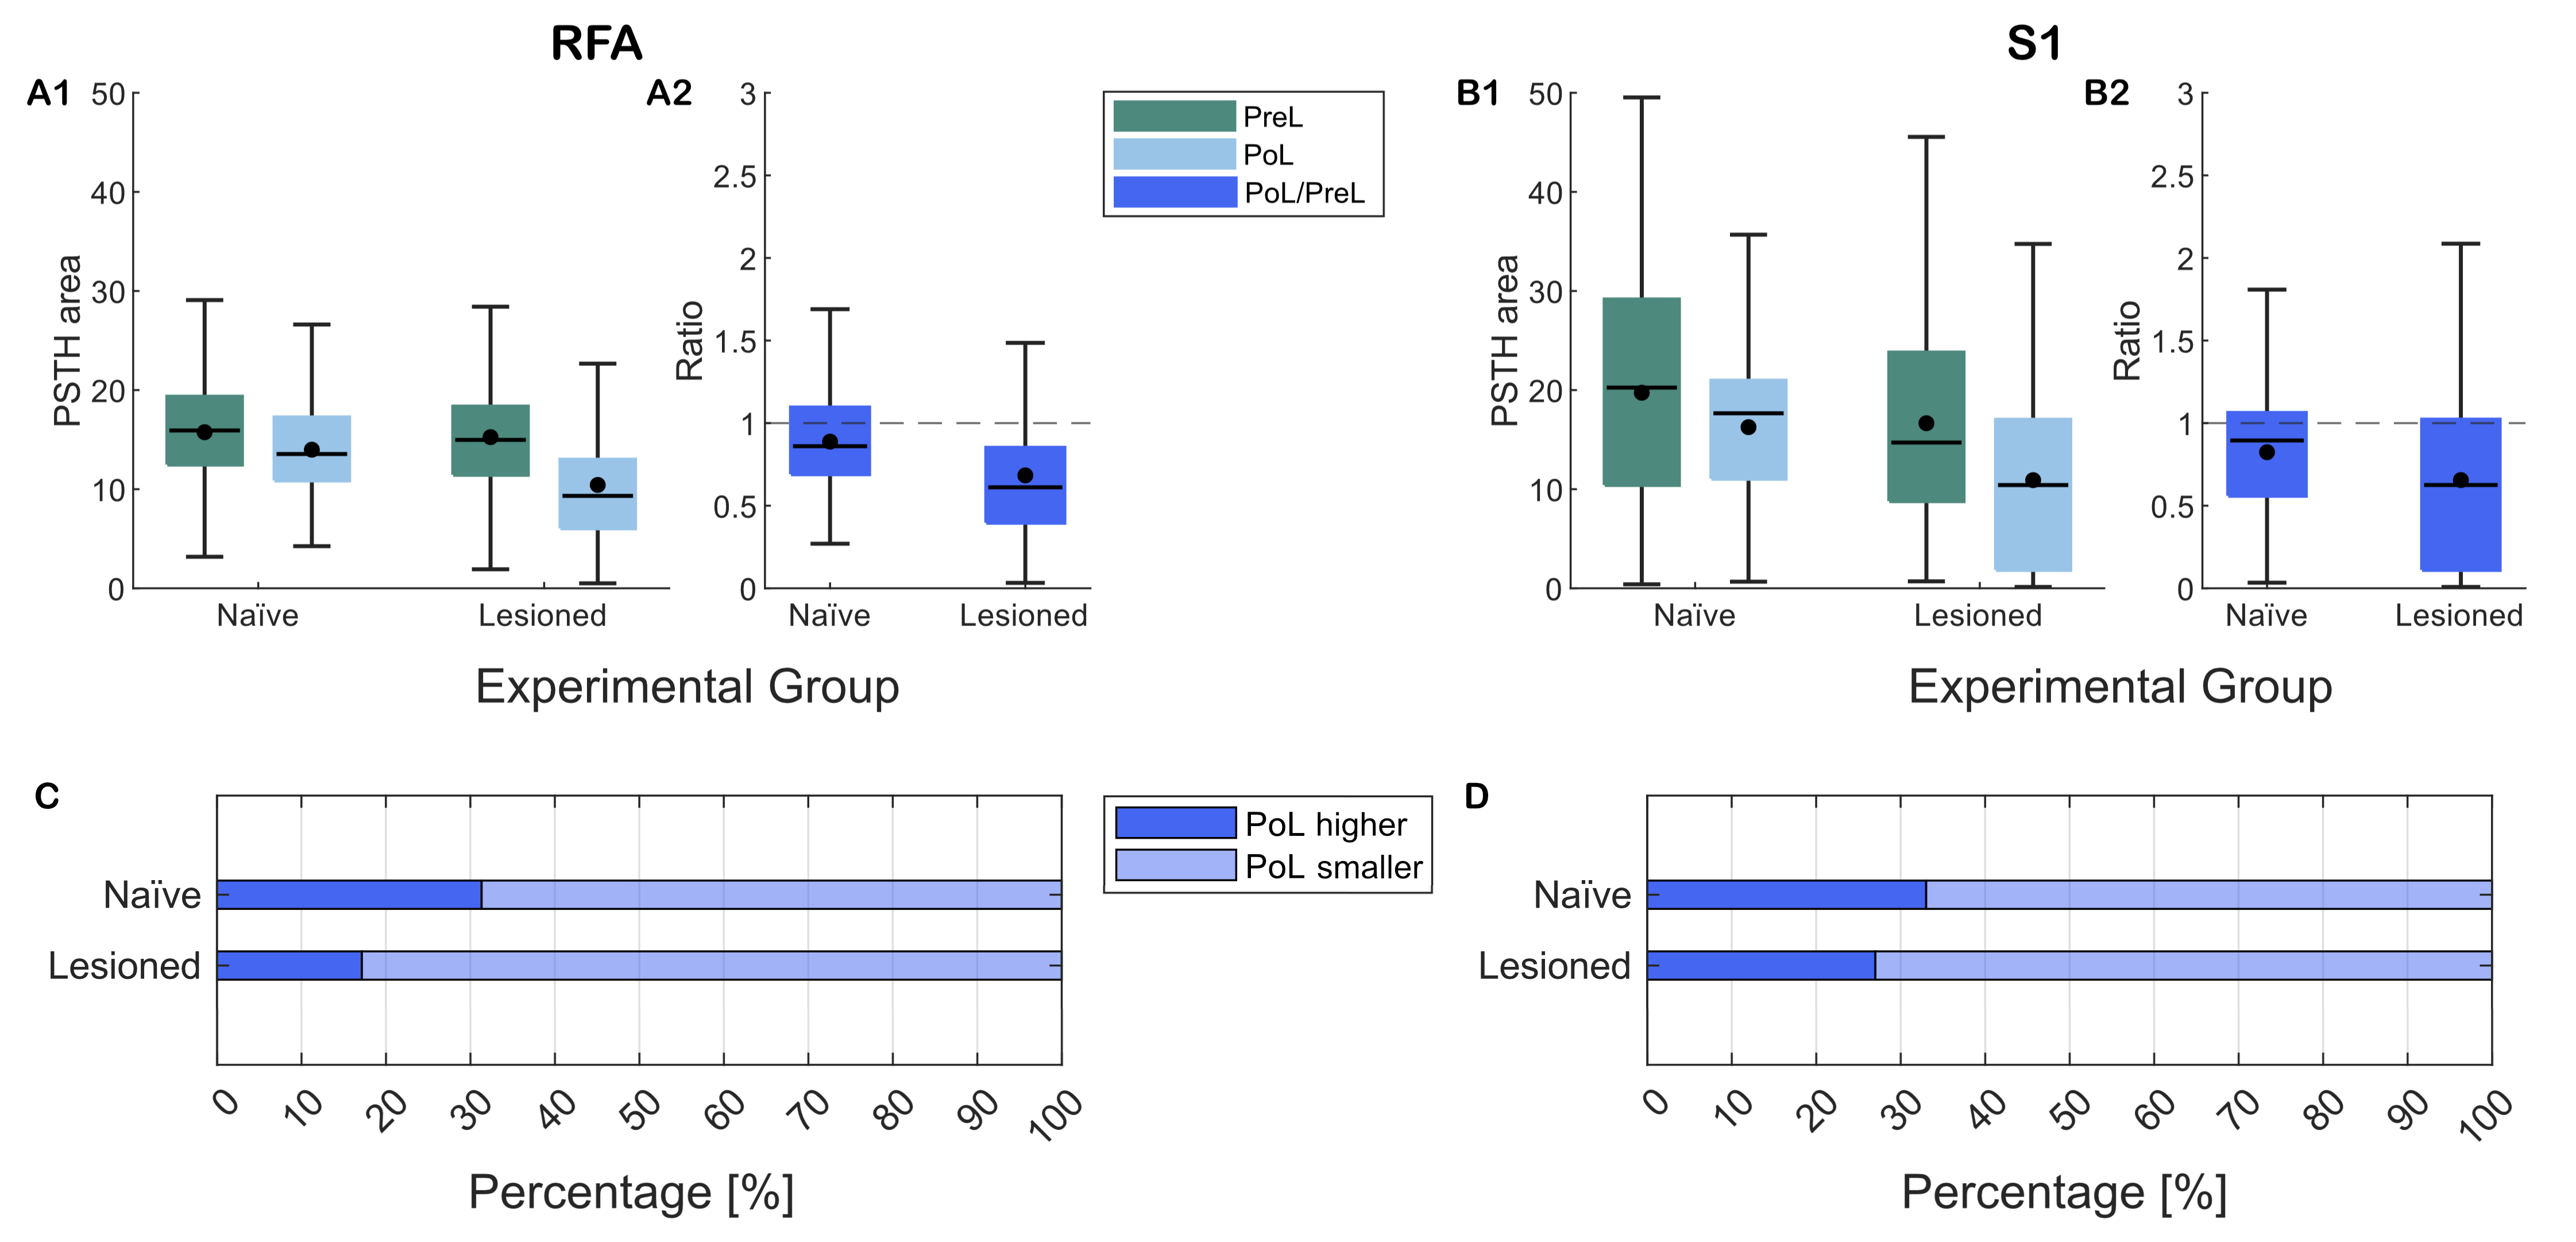
\includegraphics[width=\linewidth]{Figure/Ratio PSTH area separate/ratio PoL-PreL PSTH area 0.2Hz.jpg}
    \end{center}
    \caption{Effect of lesion on the evoked response (Connectivity Mapping stimulation 0.2Hz). (A) Box plot of the PSTH area of RFA for the entire dataset of Naïve and Lesioned rats stimulated with an OL (EXP, RS, SH) paradigm. (B) Box plot of the PSTH area of S1 for the entire dataset of Naïve and Lesioned rats stimulated with an OL (EXP, RS, SH) paradigm. (A2, B2) Box plot of the ratio between the PSTH area of the PoL phase with the mean PSTH area of the PreL phase. For each box plot (A, B), the central black line indicates the median, the central black dot indicates the mean and the box limits indicate the 25th and 75th percentiles. The whiskers show the Q1-1.5*IQR and Q3+1.5*IQR, where Q1 and Q3 are the first and third quartiles, while the IQR is the interquartile range (the distance between Q1 and Q3). (C, D) Bar plot of the percentage of channels of RFA and S1 that has an PSTH area in the PoL phase greater than the mean PSTH area in the PreL phase, for the entire dataset of Naïve and Lesioned rats stimulated with an OL (EXP, RS, SH) paradigm.}
    \label{fig:ratio PoL-PreL PSTH area 0.2Hz}
\end{figure}

\begin{figure}[ht!]
    \begin{center}
    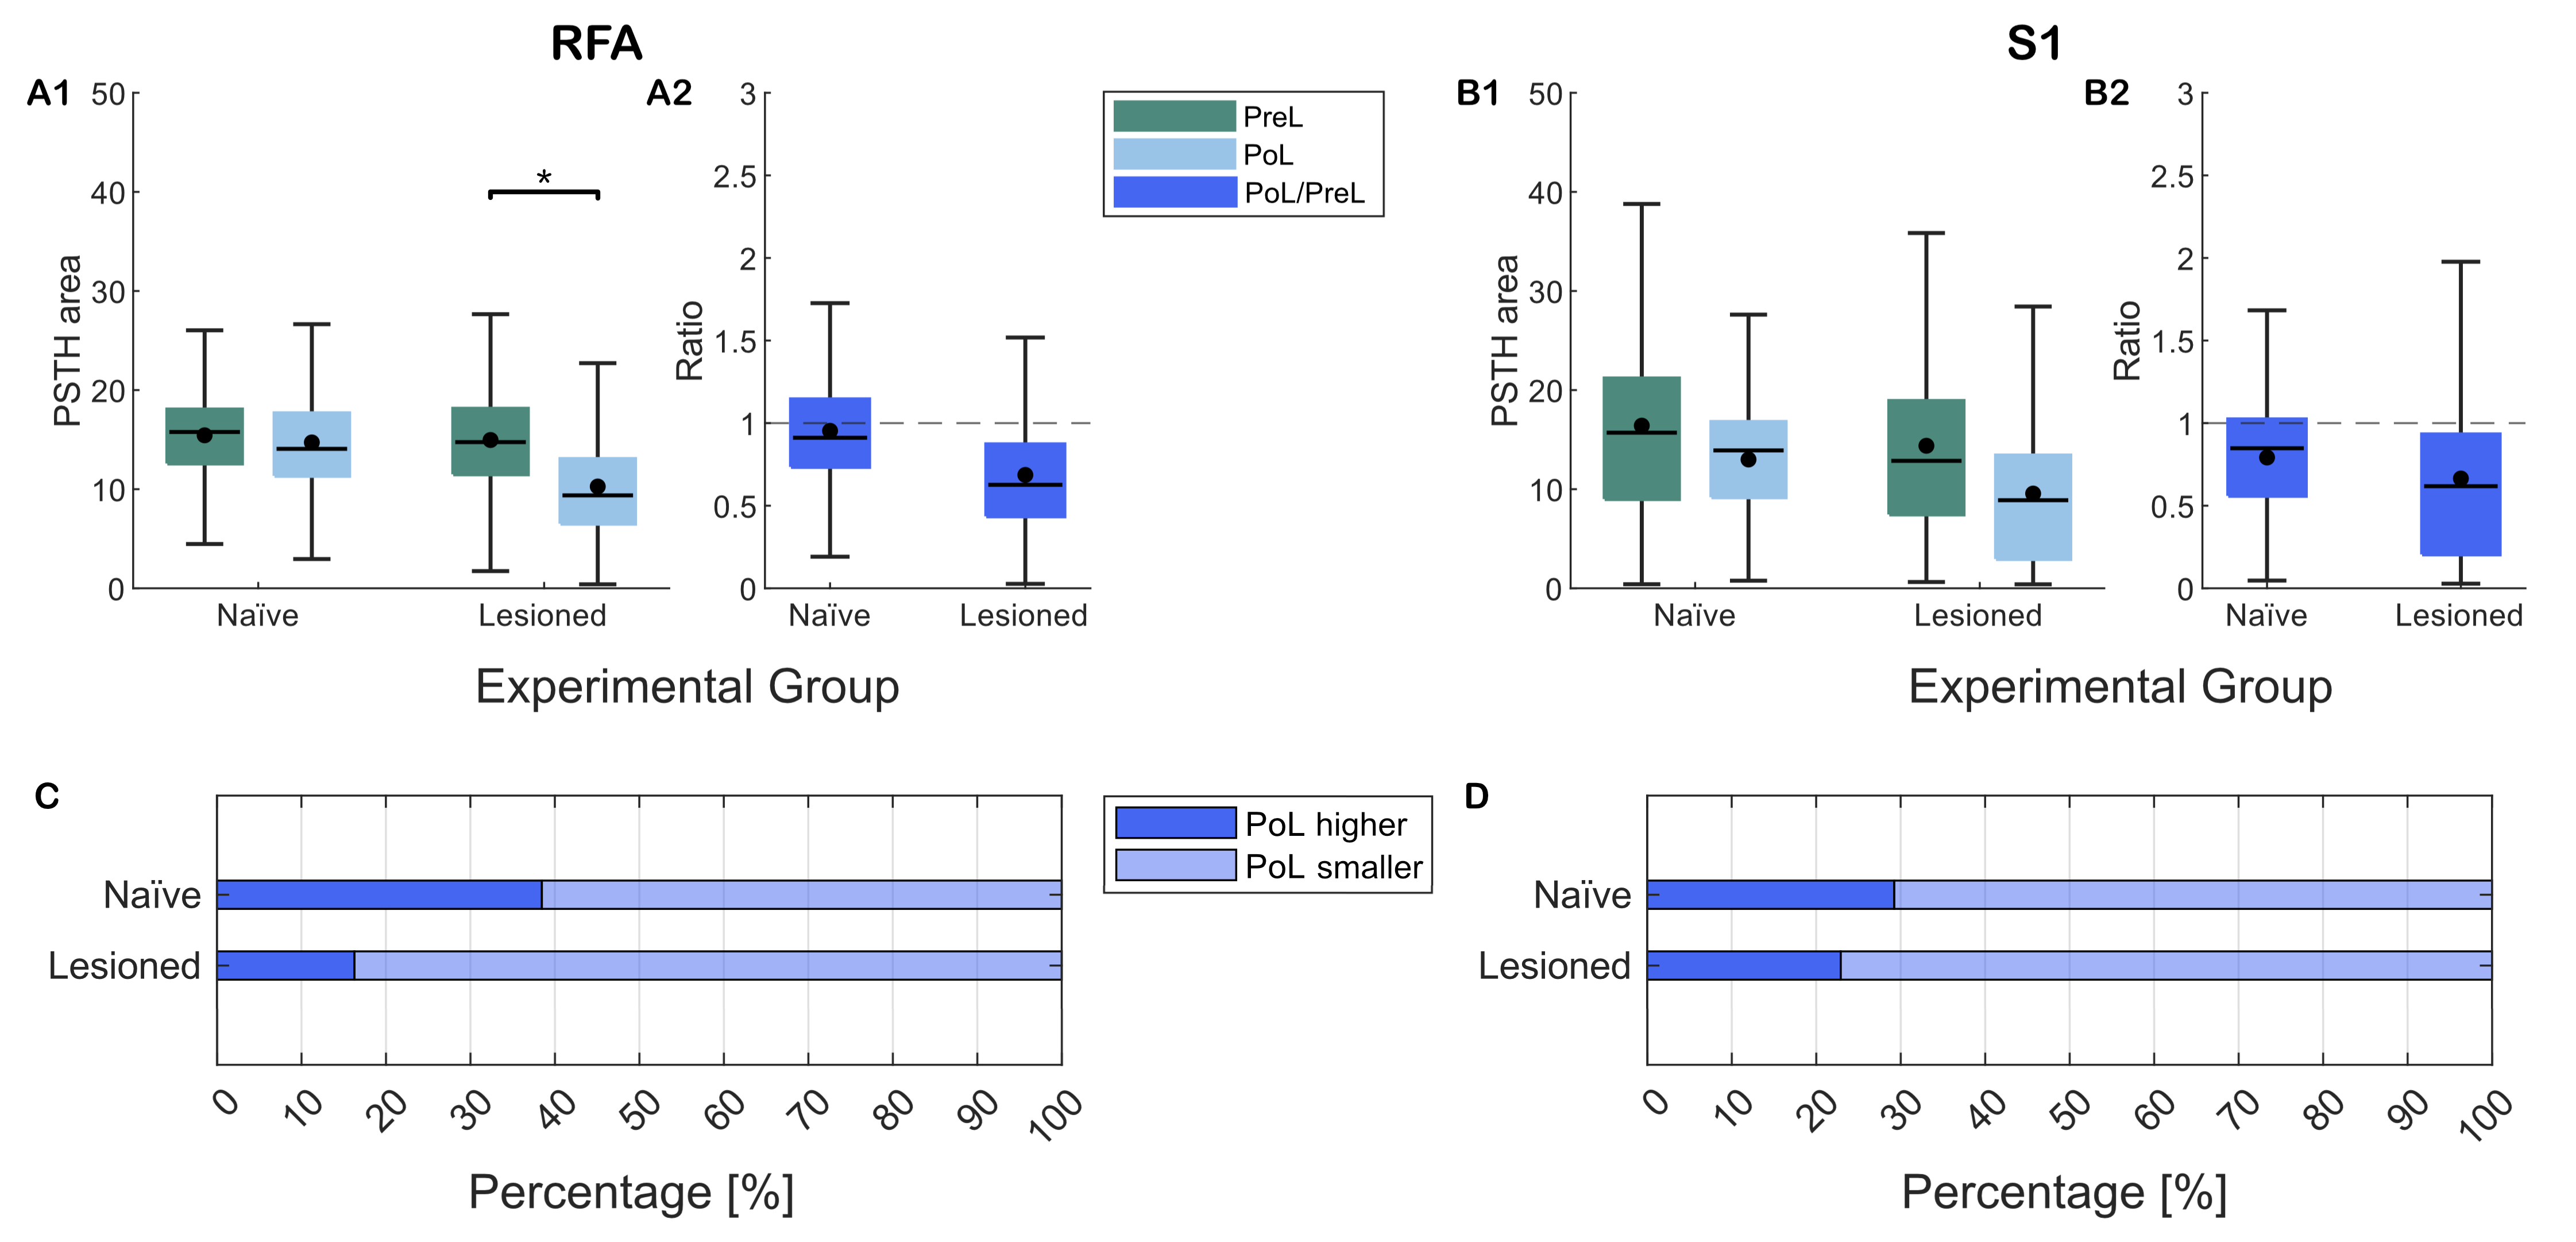
\includegraphics[width=0.90\linewidth]{Figure/Ratio PSTH area separate/ratio PoL-PreL PSTH area 1Hz.jpg}
    \end{center}
    \caption{Effect of lesion on the evoked response (Connectivity Mapping stimulation 1Hz). (A) Box plot of the PSTH area of RFA for the entire dataset of Naïve and Lesioned rats stimulated with an OL (EXP, RS, SH) paradigm. (B) Box plot of the PSTH area of S1 for the entire dataset of Naïve and Lesioned rats stimulated with an OL (EXP, RS, SH) paradigm. (A2, B2) Box plot of the ratio between the PSTH area of the PoL phase with the mean PSTH area of the PreL phase. For each box plot (A, B), the central black line indicates the median, the central black dot indicates the mean and the box limits indicate the 25th and 75th percentiles. The whiskers show the Q1-1.5*IQR and Q3+1.5*IQR, where Q1 and Q3 are the first and third quartiles, while the IQR is the interquartile range (the distance between Q1 and Q3). Solid line *: $p<0.05$, one-way ANOVA test. (C, D) Bar plot of the percentage of channels of RFA and S1 that has an PSTH area in the PoL phase greater than the mean PSTH area in the PreL phase, for the entire dataset of Naïve and Lesioned rats stimulated with an OL (EXP, RS, SH) paradigm.}
    \label{fig:ratio PoL-PreL PSTH area 1Hz}
\end{figure}

\clearpage
\subsection{The effect of the experimental procedure on the evoked responses}

The aim of this analysis was to assess the impact of the experimental procedures on evoked activity and their ability to restore the Pre-Lesion activity level.

The previous analysis revealed a global decrease in activity in both the Naïve and Lesioned groups during the Post-Lesion (PoL) phase.

Figure \ref{fig:PSTH area PreL-PoS 0.2Hz} and Figure \ref{fig:PSTH area PreL-PoS 1Hz} highlights that, even after the stimulation phase, all experimental groups (both Naïve and Lesioned) still exhibit decreased activity in both areas (RFA and S1), except for the group that received Closed Loop, Activity-Dependent Stimulation (CL: ADS), showing increased activity in the RFA area.

Focusing on the Naïve group, it is evident that the CL: ADS paradigm effectively increases the connectivity between the two areas, leveraging plasticity. In contrast, the other paradigms do not noticeably impact this interplay, as they fail to bring the activity levels back to the Pre-Lesion state.

\begin{figure}[htp]
    \begin{center}
    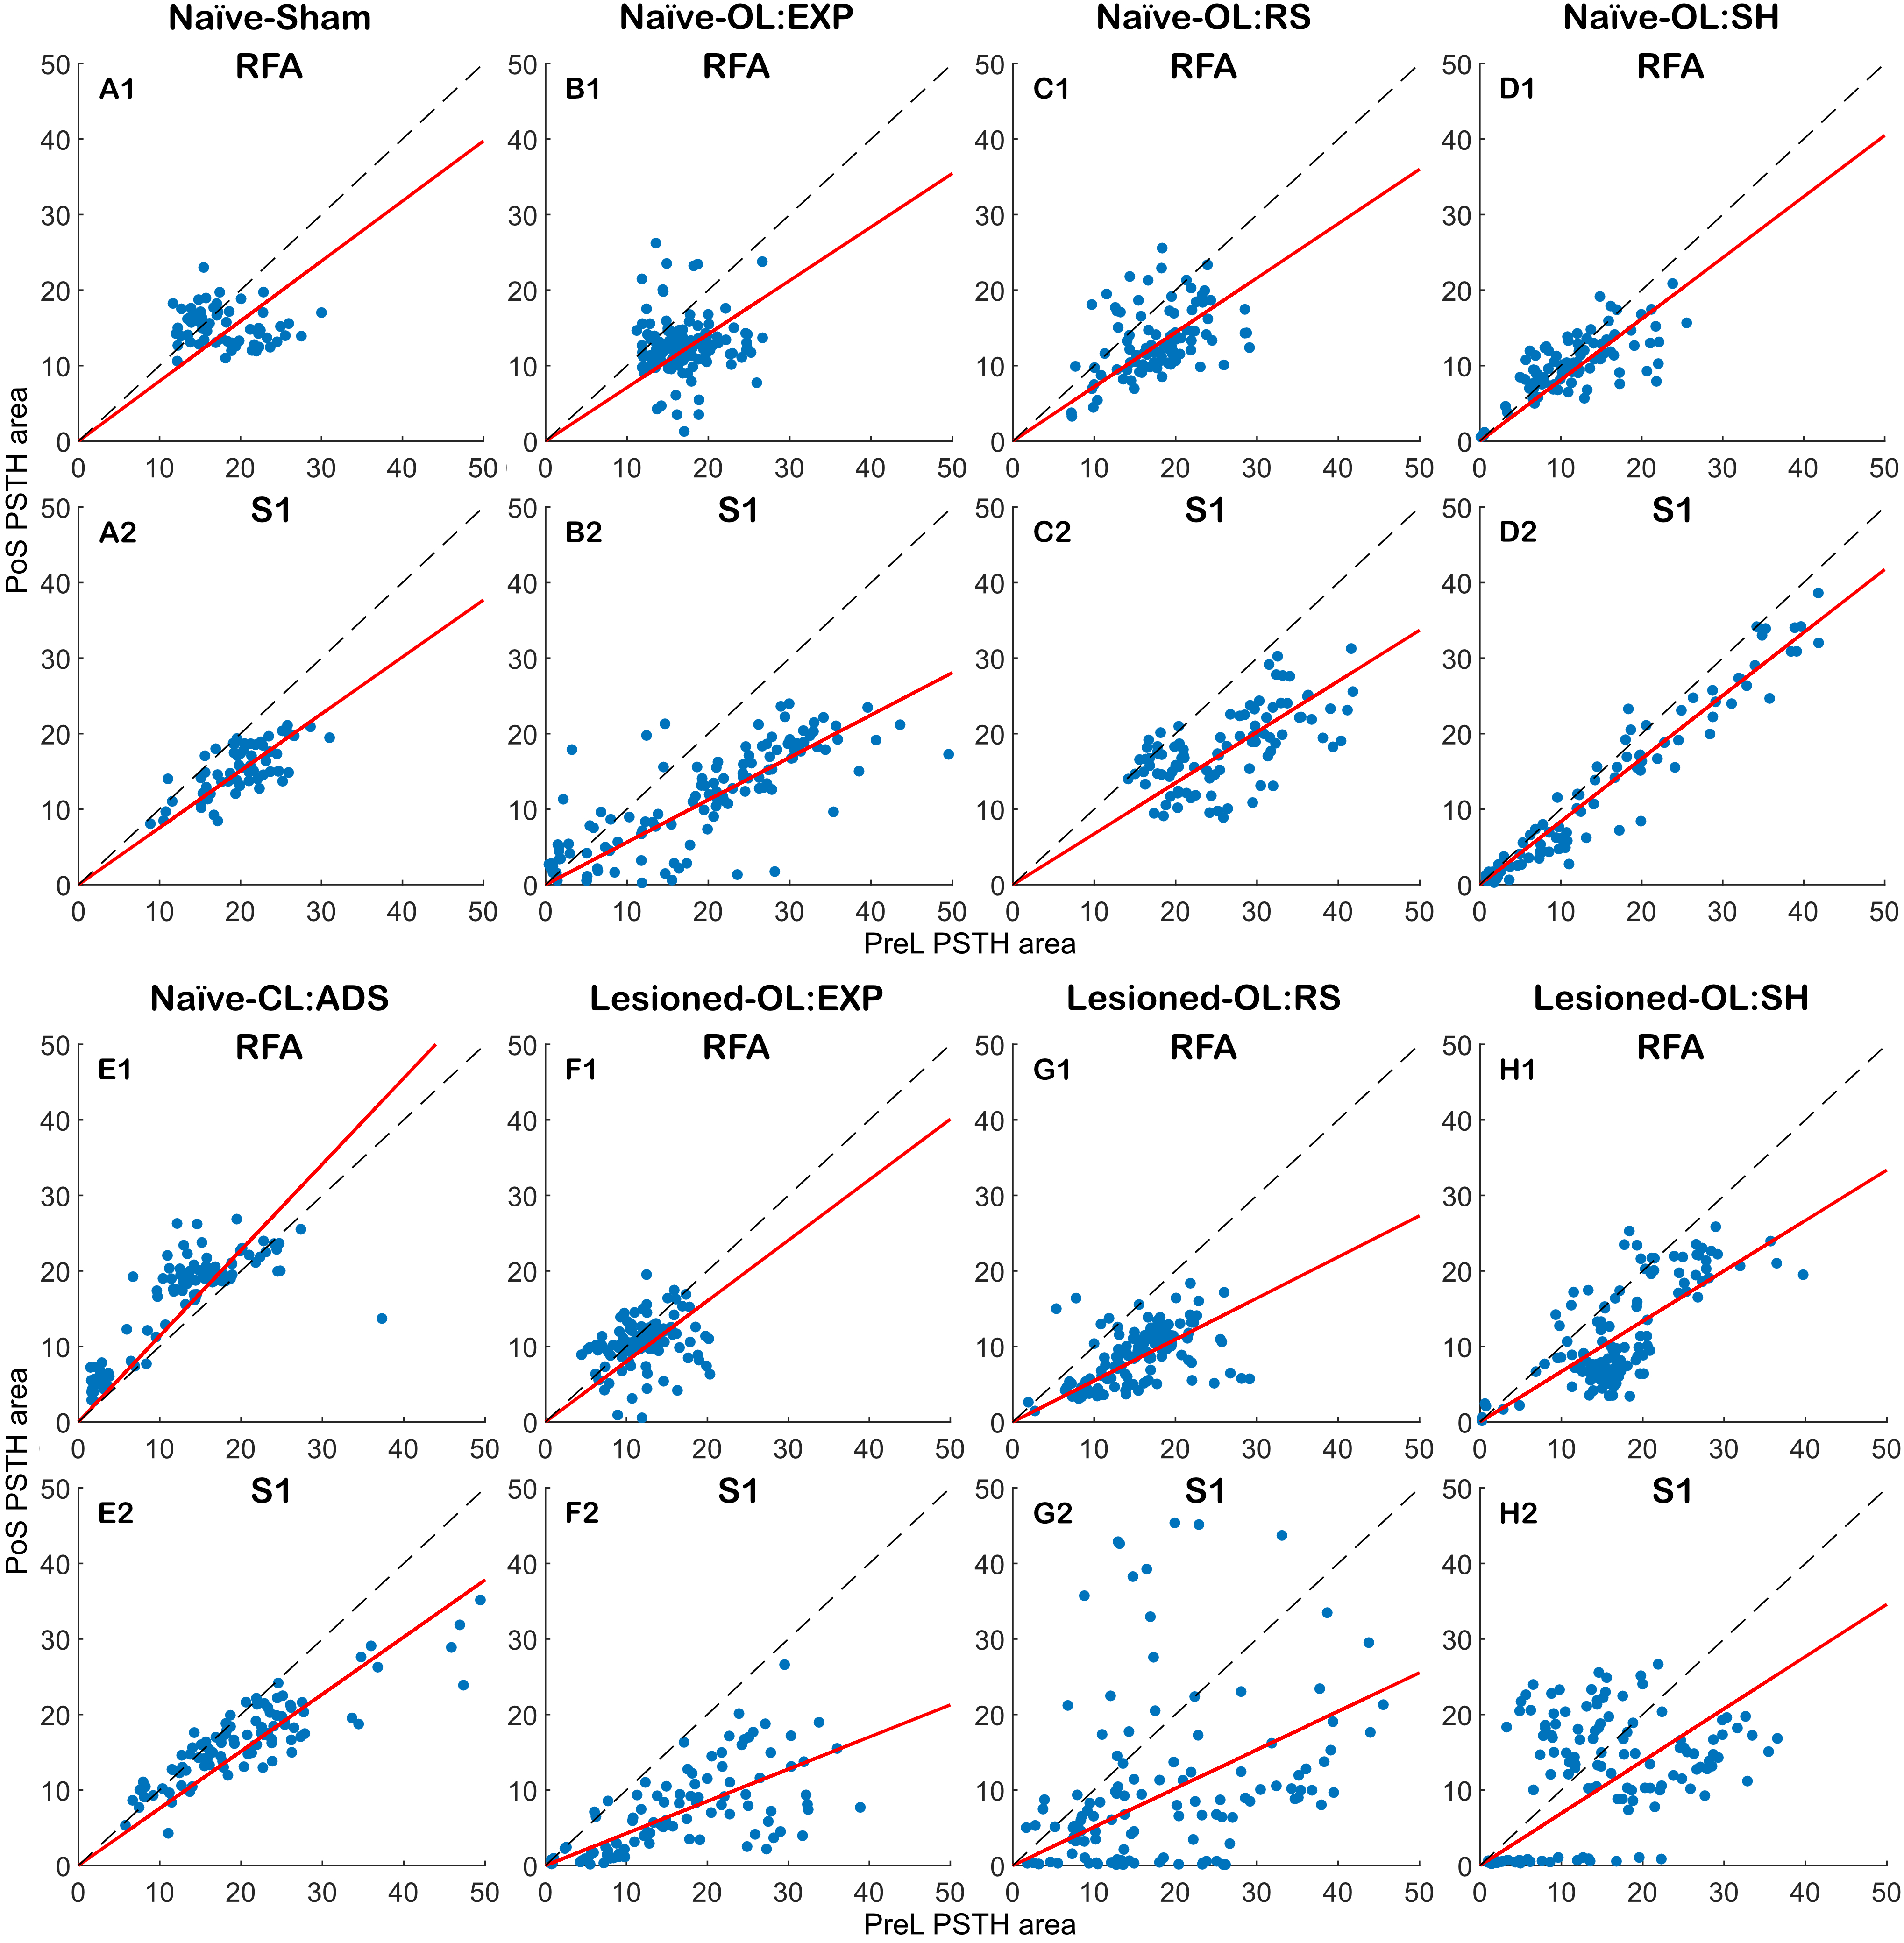
\includegraphics[width=\linewidth]{Figure/PSTH area PreL-PoS/PSTH area PreL-PoS 0.2Hz.jpg}
    \end{center}
\end{figure}
\begin{figure}[p!]
    \caption{(figure in the previous page) Pre-Lesion and Post-Stimulation PSTH area for the 0.2Hz stimulation rate. On the x-axis is showed the Pre- Lesion (PreL) PSTH area and on the y-axis the Post-Lesion (PoL) PSTH area. Each dot represent a channel. The dotted line represents the bisector with a slope of 1. The red line represent the regression line of the dots that pass through the center of axes (slopes: A1, A2: 0.79, 0.75; B1, B2: 0.71, 0.56; C1, C2: 0.72, 0.67; D1, D2: 0.81, 0.83; E1, E2: 1.14, 0.76; F1, F2: 0.80, 0.43; G1, G2: 0.55, 0.51; H1, H2: 0.67, 0.69).}
    \label{fig:PSTH area PreL-PoS 0.2Hz}
\end{figure}
\clearpage

\begin{figure}[htp]
    \begin{center}
    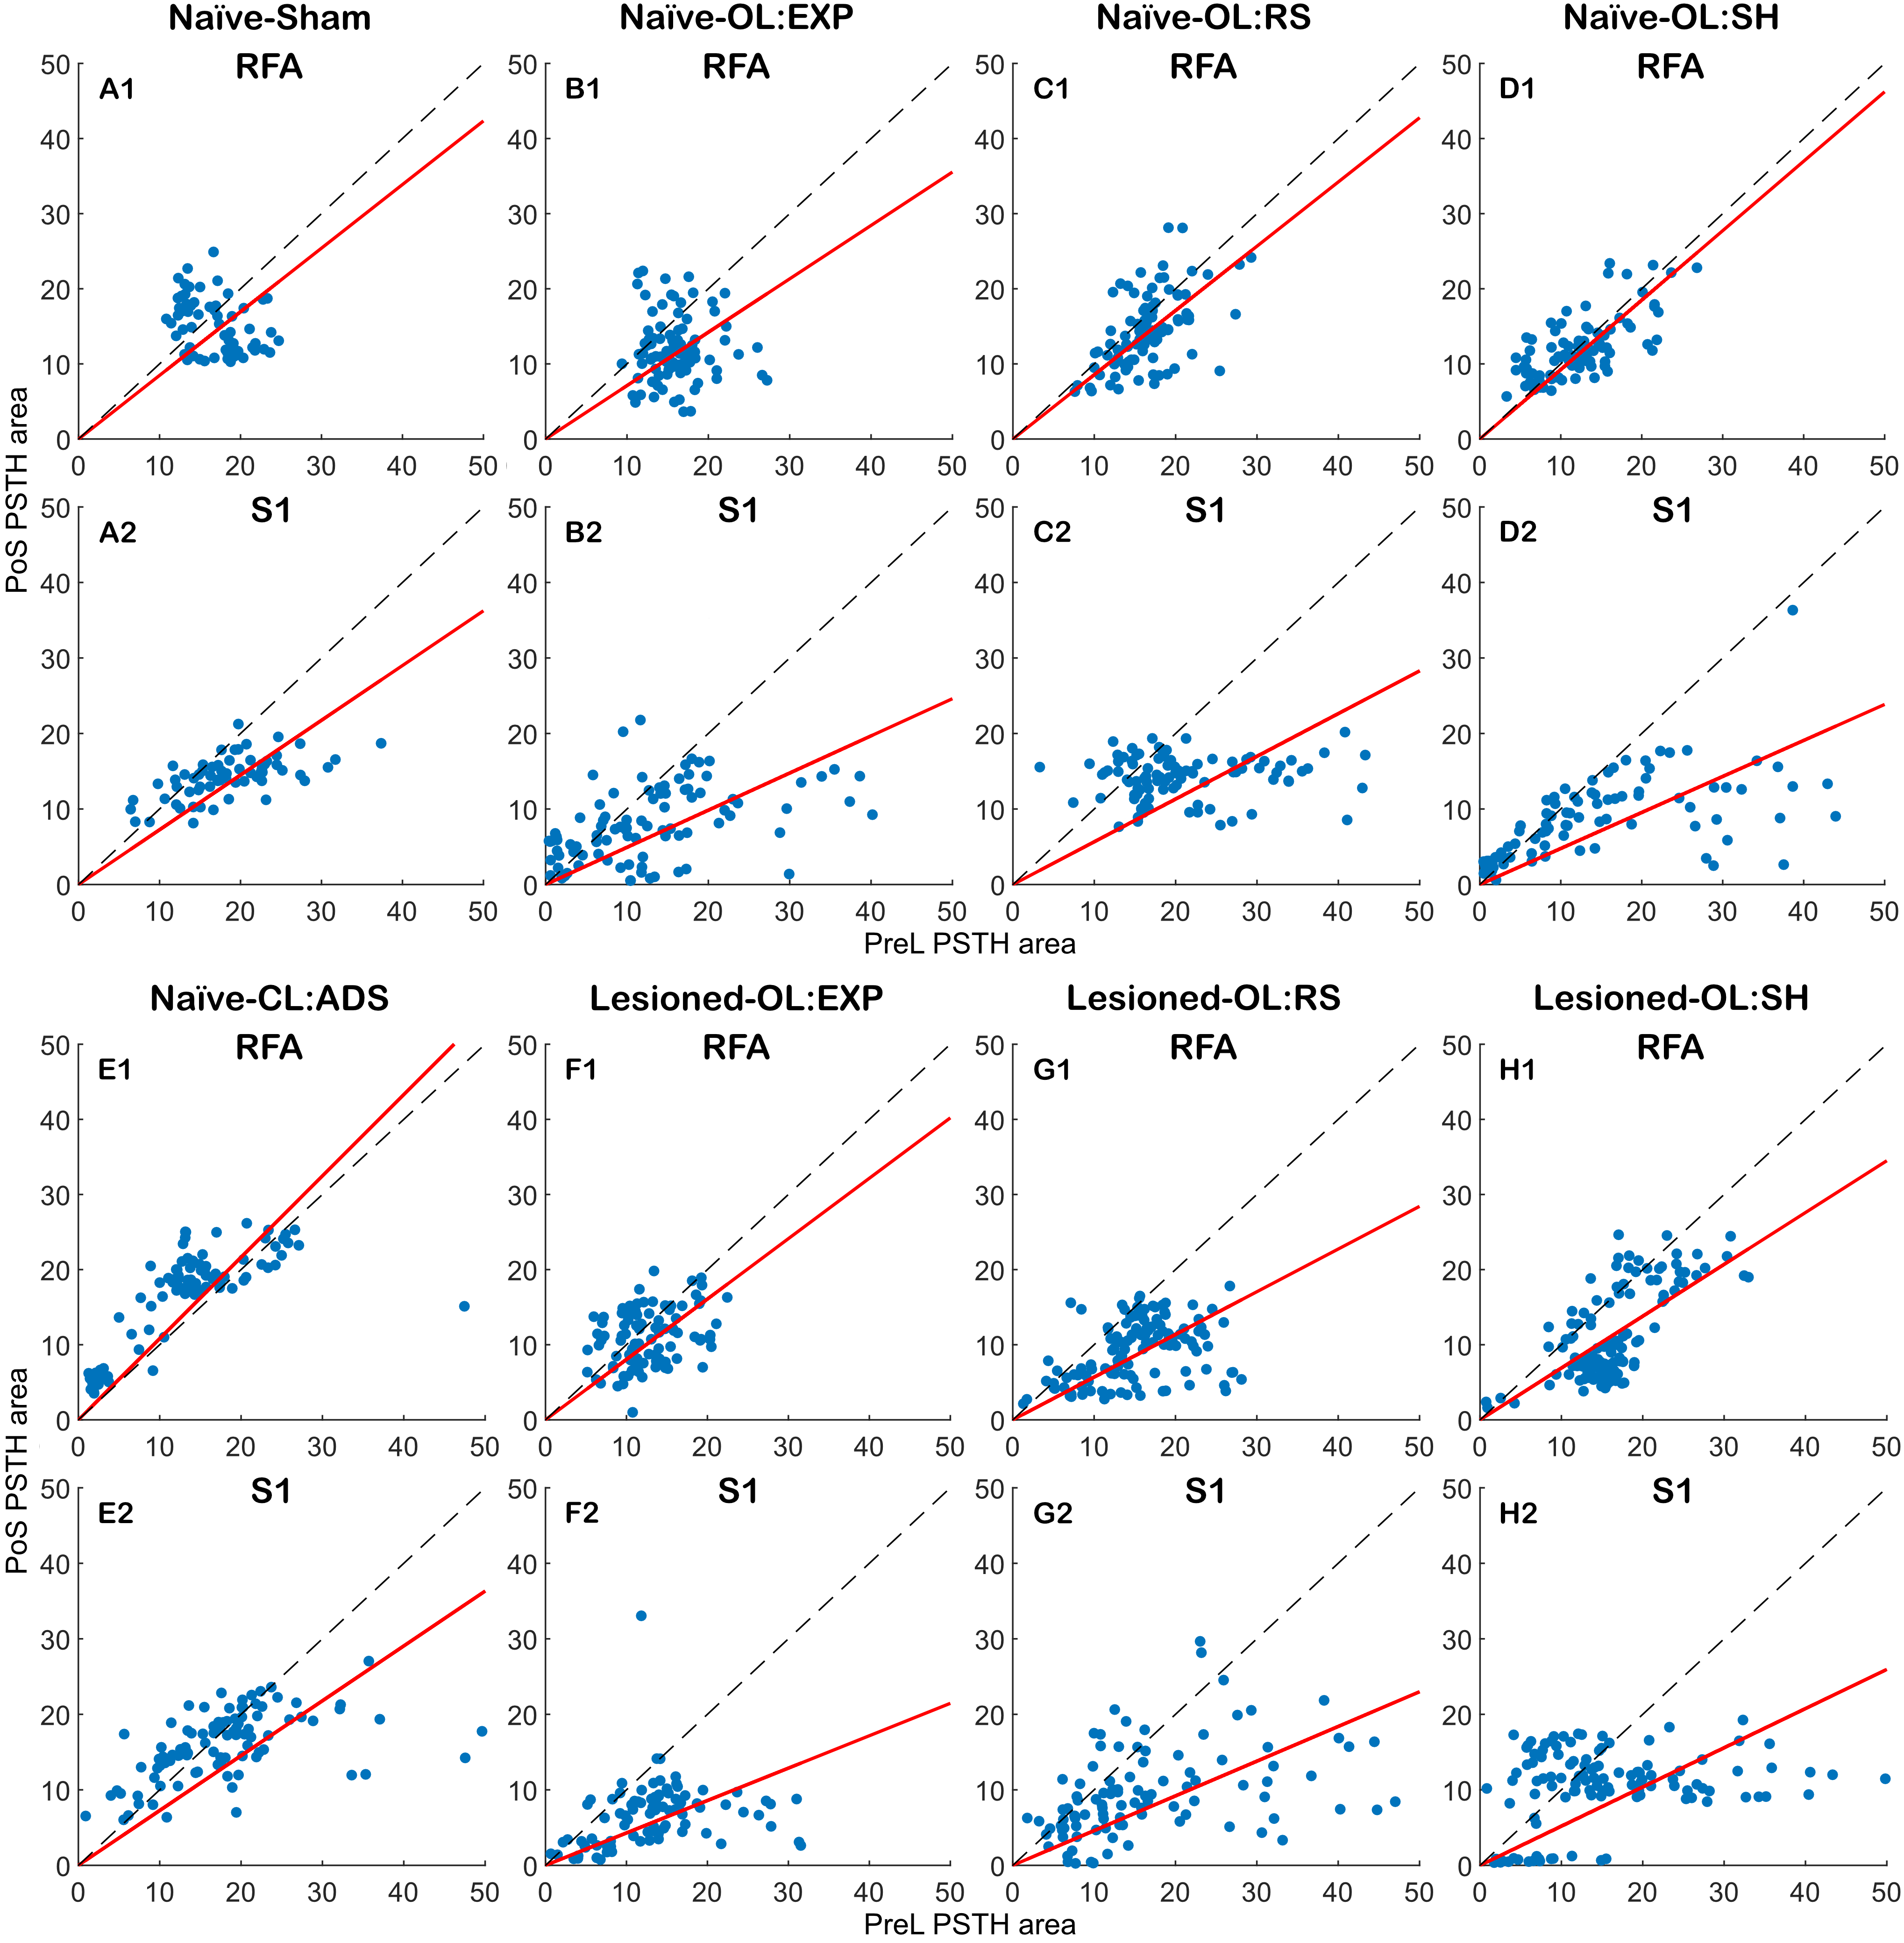
\includegraphics[width=\linewidth]{Figure/PSTH area PreL-PoS/PSTH area PreL-PoS 1Hz.jpg}
    \end{center}
\end{figure}
\begin{figure}[p!]
    \caption{(figure in the previous page) Pre-Lesion and Post-Stimulation PSTH area for the 1Hz stimulation rate. On the x-axis is showed the Pre- Lesion (PreL) PSTH area and on the y-axis the Post-Lesion (PoL) PSTH area. Each dot represent a channel. The dotted line represents the bisector with a slope of 1. The red line represent the regression line of the dots that pass through the center of axes (slopes: A1, A2: 0.85, 0.72; B1, B2: 0.71, 0.49; C1, C2: 0.86, 0.57; D1, D2: 0.92, 0.48; E1, E2: 1.08, 0.73; F1, F2: 0.80, 0.43; G1, G2: 0.57, 0.46; H1, H2: 0.69, 0.52).}
    \label{fig:PSTH area PreL-PoS 1Hz}
\end{figure}

\clearpage
\subsection{The effect of the Open Loop stimulations on the evoked responses}

In Figure \ref{fig:ratio all PSTH area 0.2Hz} and \ref{fig:ratio all PSTH area 1Hz}, it is depicted how the area under the PSTH keeps decreasing, even after the stimulation protocol, in the majority of the cases. However there are no significant differences between the PreL, PoL and PoS phases.

Analyzing the effect of the stimulation on the Naïve animals, it's evident that in all the cases this leads to a further decrease of the evoked response, in addition to the decrease yield by the lesion (Figure \ref{fig:ratio all PSTH area 0.2Hz} and \ref{fig:ratio all PSTH area 1Hz}). This behaviour is not always true in the lesioned animals, where the OL: SH paradigms leads to more channels with an higher evoked activity in S1 (Figure \ref{fig:ratio all PSTH area 0.2Hz} E, F, G, H) or RFA(Figure \ref{fig:ratio all PSTH area 1Hz} E, F, G, H) compared to the PreL phase.

\begin{figure}[htp]
    \begin{center}
    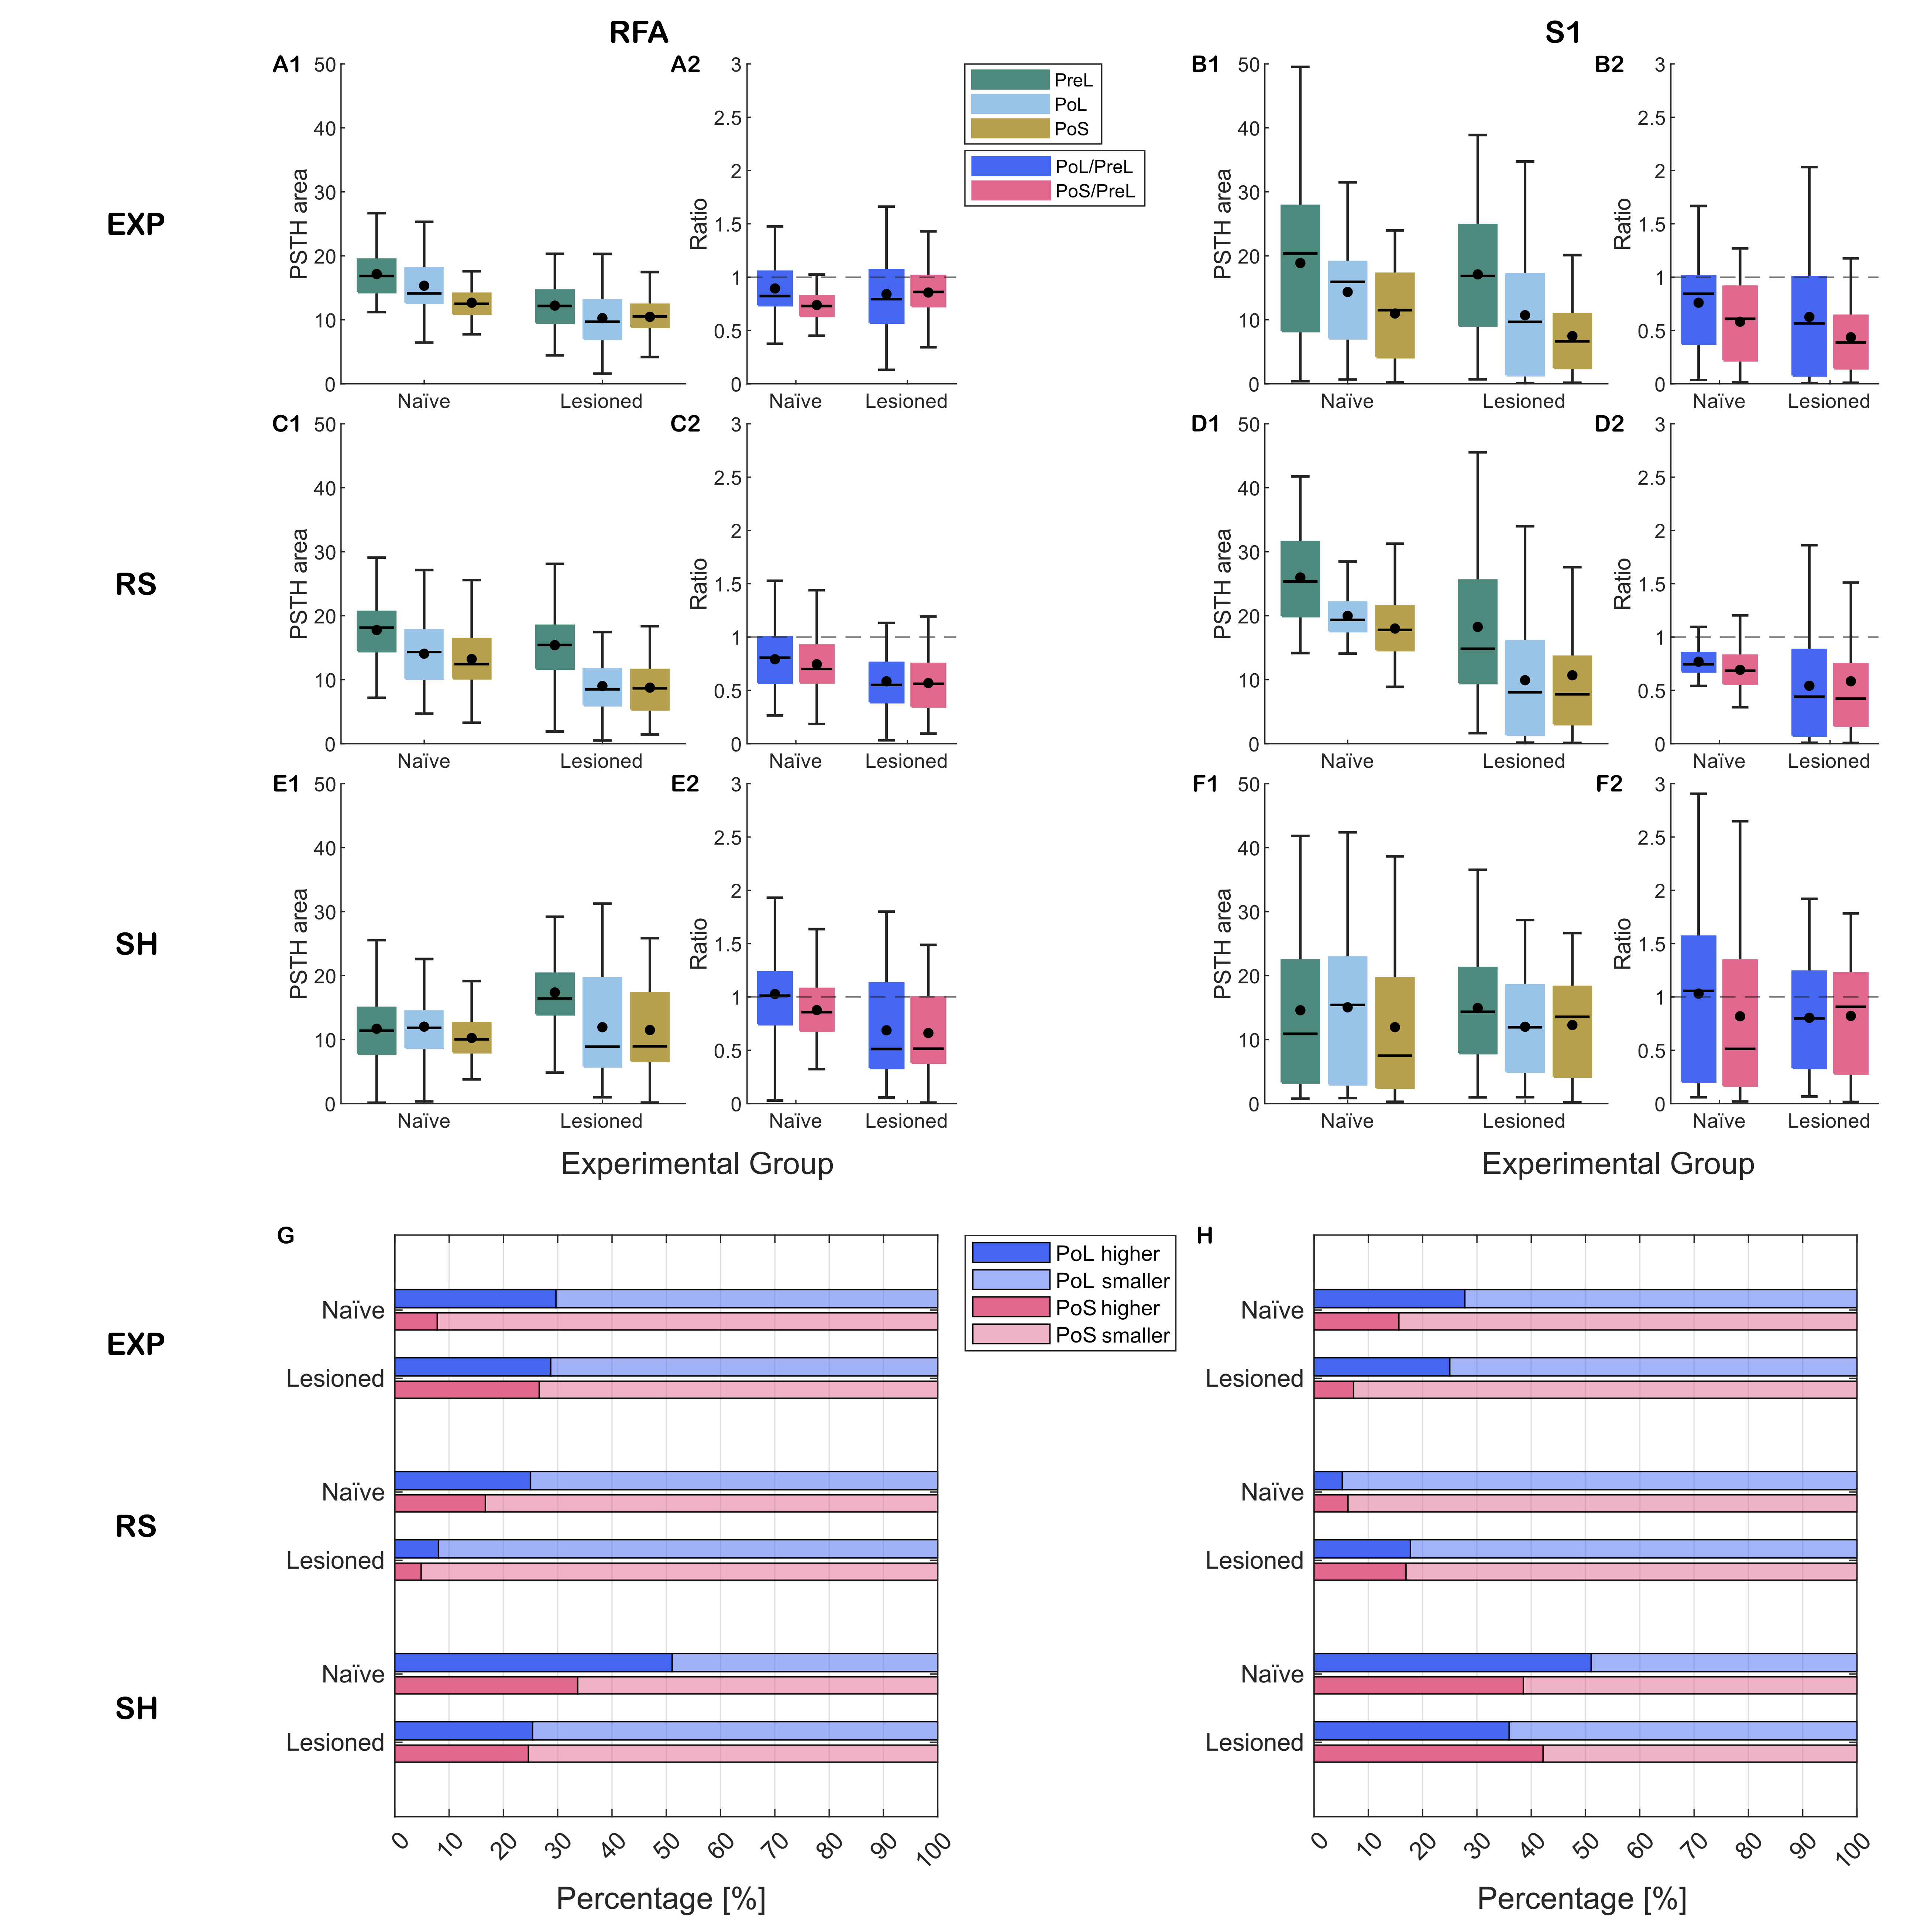
\includegraphics[width=\linewidth]{Figure/Ratio PSTH area separate/ratio all PSTH area 0.2Hz.jpg}
    \end{center}
\end{figure}
\begin{figure}[p!]
    \caption{(figure in the previous page) Effect of lesion and OL stimulations on the evoked response (Connectivity Mapping stimulation 0.2Hz). (A, C, E) Box plot of the PSTH area of RFA for the entire dataset of Naïve and Lesioned rats stimulated with an OL (EXP, RS, SH) paradigm. (B, D, F) Box plot of the PSTH area of S1 for the entire dataset of Naïve and Lesioned rats stimulated with an OL (EXP, RS, SH) paradigm. (A2, B2, C2, D2, E2, F2) Box plot of the ratio between the PSTH area of the PoL and PoS phases with the mean PSTH area of the PreL phase. For each box plot (A - F), the central black line indicates the median, the central black dot indicates the mean and the box limits indicate the 25th and 75th percentiles. The whiskers show the Q1-1.5*IQR and Q3+1.5*IQR, where Q1 and Q3 are the first and third quartiles, while the IQR is the interquartile range (the distance between Q1 and Q3). (G, H) Bar plot of the percentage of channels of RFA and S1 that has an PSTH area in the PoL and PoS phases greater than the mean PSTH area in the PreL phase, for the entire dataset of Naïve and Lesioned rats stimulated with an OL (EXP, RS, SH) paradigm.}
    \label{fig:ratio all PSTH area 0.2Hz}
\end{figure}
\clearpage

\begin{figure}[htp]
    \begin{center}
    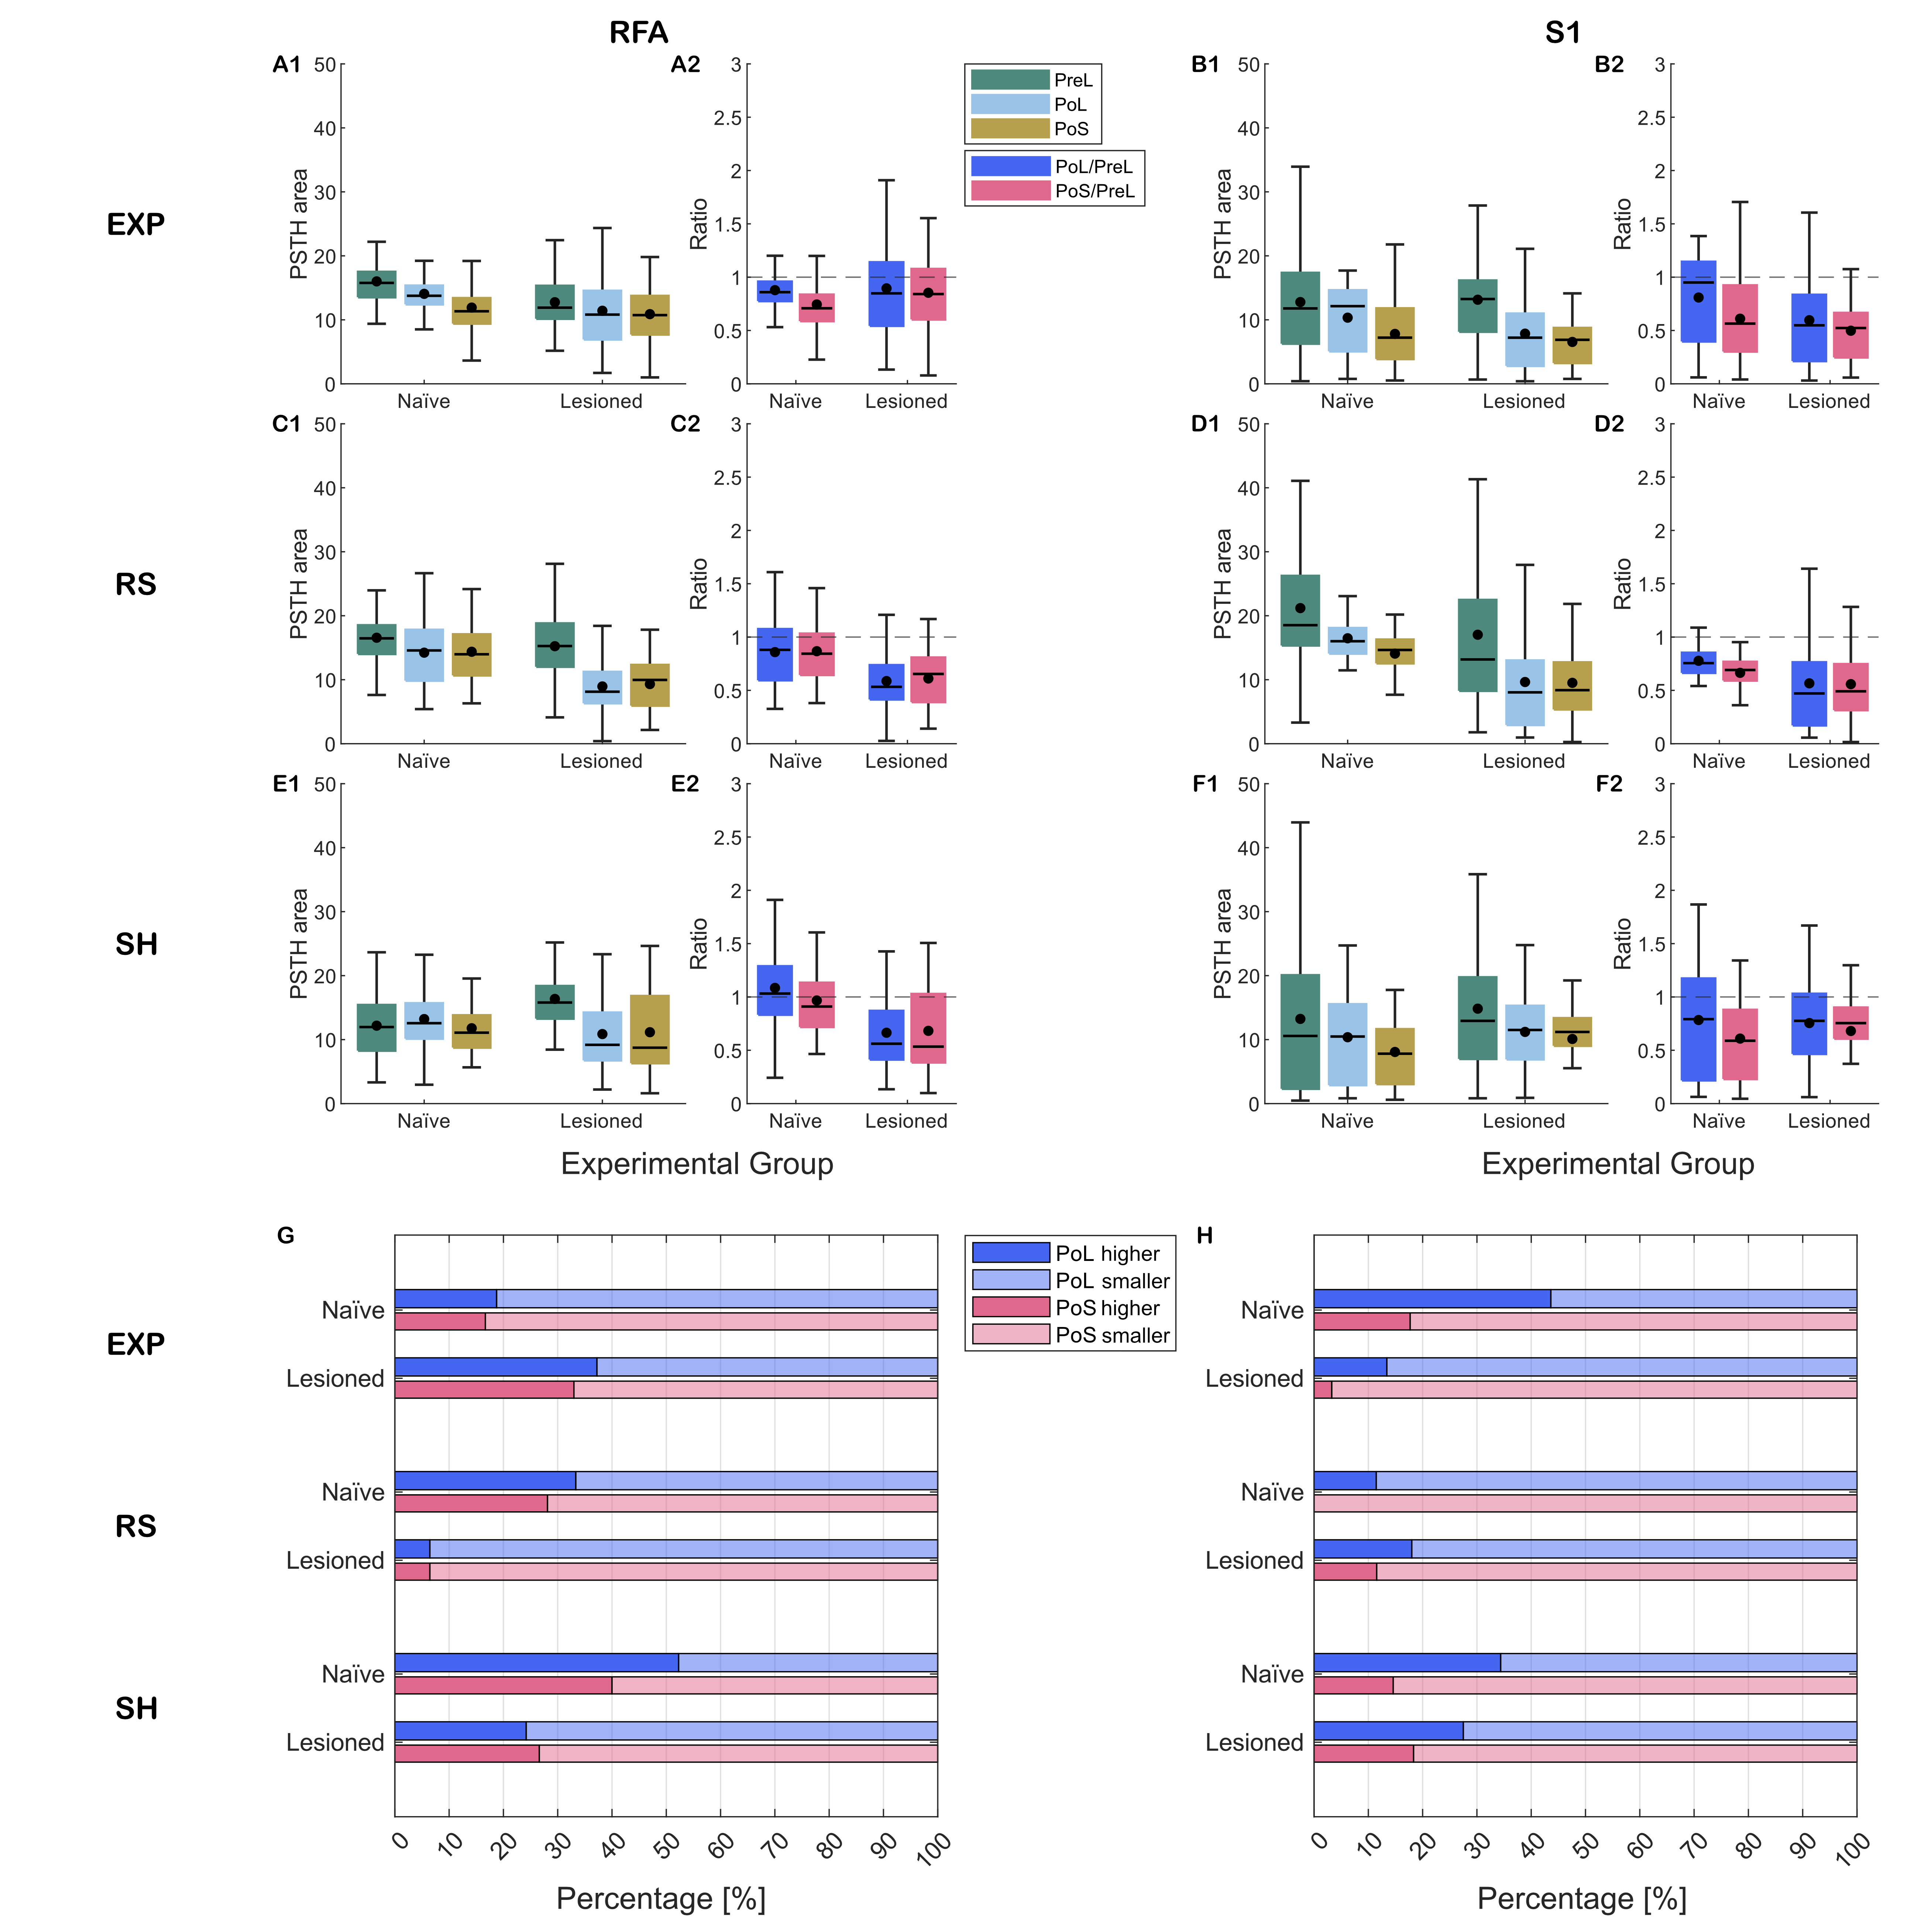
\includegraphics[width=\linewidth]{Figure/Ratio PSTH area separate/ratio all PSTH area 1Hz.jpg}
    \end{center}
\end{figure}
\begin{figure}[p!]
    \caption{(figure in the previous page) Effect of lesion and OL stimulations on the evoked response (Connectivity Mapping stimulation 1Hz). (A, C, E) Box plot of the PSTH area of RFA for the entire dataset of Naïve and Lesioned rats stimulated with an OL (EXP, RS, SH) paradigm. (B, D, F) Box plot of the PSTH area of S1 for the entire dataset of Naïve and Lesioned rats stimulated with an OL (EXP, RS, SH) paradigm. (A2, B2, C2, D2, E2, F2) Box plot of the ratio between the PSTH area of the PoL and PoS phases with the mean PSTH area of the PreL phase. For each box plot (A - F), the central black line indicates the median, the central black dot indicates the mean and the box limits indicate the 25th and 75th percentiles. The whiskers show the Q1-1.5*IQR and Q3+1.5*IQR, where Q1 and Q3 are the first and third quartiles, while the IQR is the interquartile range (the distance between Q1 and Q3). (G, H) Bar plot of the percentage of channels of RFA and S1 that has an PSTH area in the PoL and PoS phases greater than the mean PSTH area in the PreL phase, for the entire dataset of Naïve and Lesioned rats stimulated with an OL (EXP, RS, SH) paradigm.}
    \label{fig:ratio all PSTH area 1Hz}
\end{figure}

\clearpage
\section{Discussion and Conclusion}

In this work, the electrophysiological activity of both the premotor (RFA) and somatosensory (S1) cortex in anesthetized rats affected by a focal lesion in the motor area (M1) was analyzed. The impact of the lesion and subsequent neuromodulation therapies on the evoked responses was evaluated through the computation of the Post-Stimulus Time Histogram (PSTH).

It has been observed that the lesion results in a greater decrease in evoked activity compared to the Naïve group. The CL: ADS paradigm was the only one that led to an increase in evoked activity in the PoS period with respect to the PreL, eventhough it was applied to the Naïve rats. On the other hand, all the open loop stimulation paradigms produced a further decrease of the evoked activity in all Naïve animals, and also in the lesioned ones, except for the OL: SH group.

This preliminary analysis was a necessary step to assess the effectiveness of a new form of neuromodulation therapy, where an open loop system will be utilized to deliver personalized stimulation.